
\documentclass{article}

\usepackage[ngerman]{babel}                     %for german umlauts
\usepackage[utf8]{inputenc}
\usepackage{subfigure}
\usepackage{float}
%\usepackage[framed,autolinebreaks,useliterate]{mcode}
%\usepackage[bw,framed,autolinebreaks,useliterate]{mcode}
% \usepackage[ansinew]{inputenc}        %for german umlauts

\usepackage{listings}

\usepackage{graphicx}
\usepackage{hyperref}

\usepackage{amssymb}    %for different fonts
\usepackage{amsmath}
% Geht nicht: \usepackage{bbm}
% \usepackage[usenames,dvips]{color} %only way to get it running with pdf:(
% \usepackage[pdftex,usenames,dvipsnames]{color}        % does not work
% \usepackage{color}
\usepackage{verbatim}
\usepackage{polynom}

\setlength{\parindent}{0pt}
\addtolength{\hoffset}{-2cm}
\addtolength{\voffset}{-1cm}
\addtolength{\textheight}{3cm}
\addtolength{\textwidth}{3cm}

\newcommand{\im}{\operatorname{Im}}
\newcommand{\rg}{\operatorname{rg}}
\newcommand{\ggt}{\operatorname{ggT}}

\lstset{ %
  language=Matlab,                % the language of the code
  frame=single,                   % adds a frame around the code
  tabsize=2,
  basicstyle=\footnotesize
}

\begin{document}

\section*{\begin{center} Mustererkennung - Aufgabenblatt 10 \end{center}}
\begin{center}
  André Hacker und Dimitri Schachmann \\
\end{center}

\subsection*{1. NMF}
\subsubsection*{Implementierung}
Wir haben den NMF Algorithmus in Matlab implementiert. Dabei haben wir
zwei Implementierungen erstellt. Eine die einfach zu implementieren
war und eine mit viel repmat-Magic, die dafür viel effizienter
ist:
\begin{lstlisting}
function [W H] = nmf(V, w_size, num_of_iterations)
  % random start values
  W = rand(size(V,1),w_size);
  H = rand(size(W,2),size(V,2));

  % repmat magic utility
  H_rep_index = reshape(repmat([1:size(H,1)],size(V,1),1),1,[]);
  V_rep_index = reshape(repmat([1:size(V,2)],size(W,2),1),1,[]);
  
  for i = 1:num_of_iterations
    [i num_of_iterations]
    % compute current prediction
    V_dash = W * H;
    % compute quotien between current prediction and actual image
    V_by_V = V./V_dash;

    % repmat magic utility
    V_by_V_dash = repmat(sum(V_by_V,2),1,size(W,2));
    
    % recompute W
    tmp1 = repmat(V_by_V,size(H,1),1);
    tmp2 = H(H_rep_index,:);
    big_sum = reshape(sum(tmp1 .* tmp2,2),size(W));
    W = W .* big_sum;
    
    % normalize W
    sigma_W = repmat(sum(W,1),size(W,1),1);
    W = W./sigma_W;

    % repmat magic
    tmp1 = repmat(W,1,size(V,2));
    tmp2 = V_by_V(:,V_rep_index);
    big_sum = reshape(sum(tmp1 .* tmp2,1),size(H));

    % recompute H
    H = H .* big_sum;
  end
end


function [W H] = nmf2(V, w_size, num_of_iterations)
  W = rand(size(V,1),w_size);
  H = rand(size(W,2),size(V,2));
  
  for k = 1:num_of_iterations
    V_dash = W * H;
    V_by_V = V./V_dash;
    factor = zeros(size(W));
    for i = [1:size(W,1)]
      for a = [1:size(W,2)]
        for mu = [1:size(H,2)]
          factor(i,a) = factor(i,a) + (V_by_V(i,mu) * H(a,mu));
        end
      end
    end
    W = W .* factor;
    
    sigma_W = repmat(sum(W,1),size(W,1),1);
    W = W./sigma_W;

    factor = zeros(size(H));
    for a = [1:size(W,2)]
      for mu = [1:size(H,2)]
        for i = [1:size(W,1)]
          factor(a,mu) = factor(a,mu) + (W(i,a) * V_by_V(i,mu));
        end
      end
    end
    H = H .* factor;
  end
end
\end{lstlisting}
\newpage
\subsubsection*{Ein paar Bilder und deren Rekonstruktionen 1000 Iterationen 20 Codewörter}
Im Folgenden sieht man in 2 Doppelreihen die ersten 8 Originalen Bilder (jeweils
oben) und die zugehörigen Rekonstruktionen (jeweils unten).\\
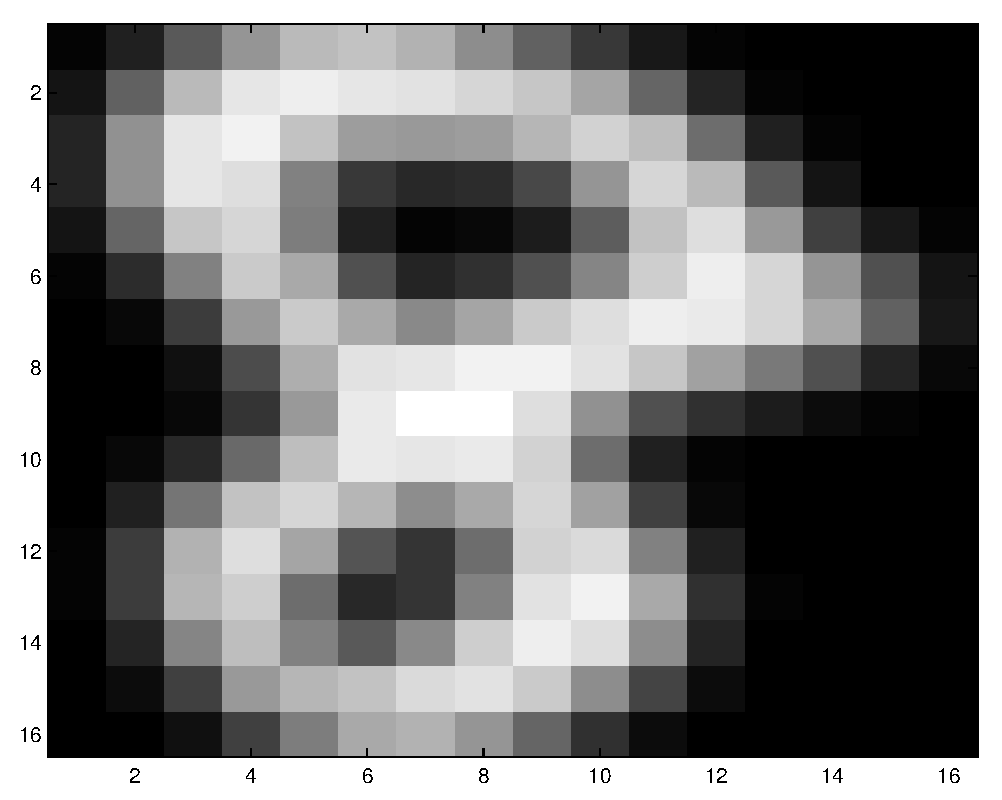
\includegraphics[width=0.25\textwidth]{digits1.eps}\hspace{0.03\textwidth}%
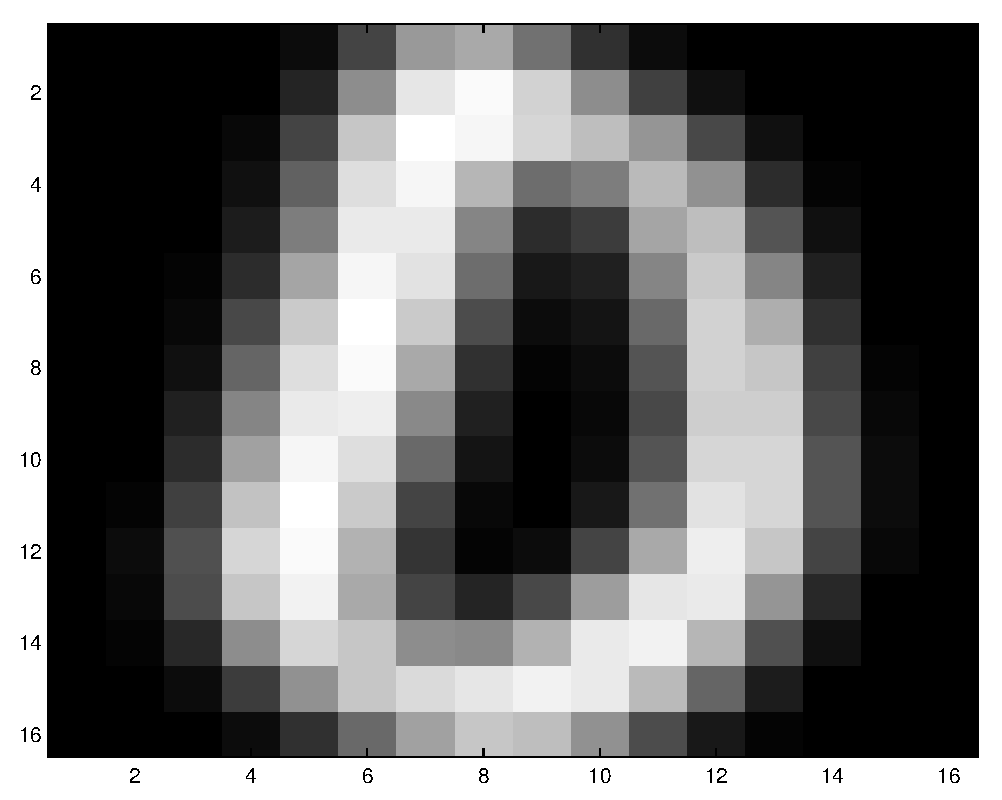
\includegraphics[width=0.25\textwidth]{digits2.eps}\hspace{0.03\textwidth}%
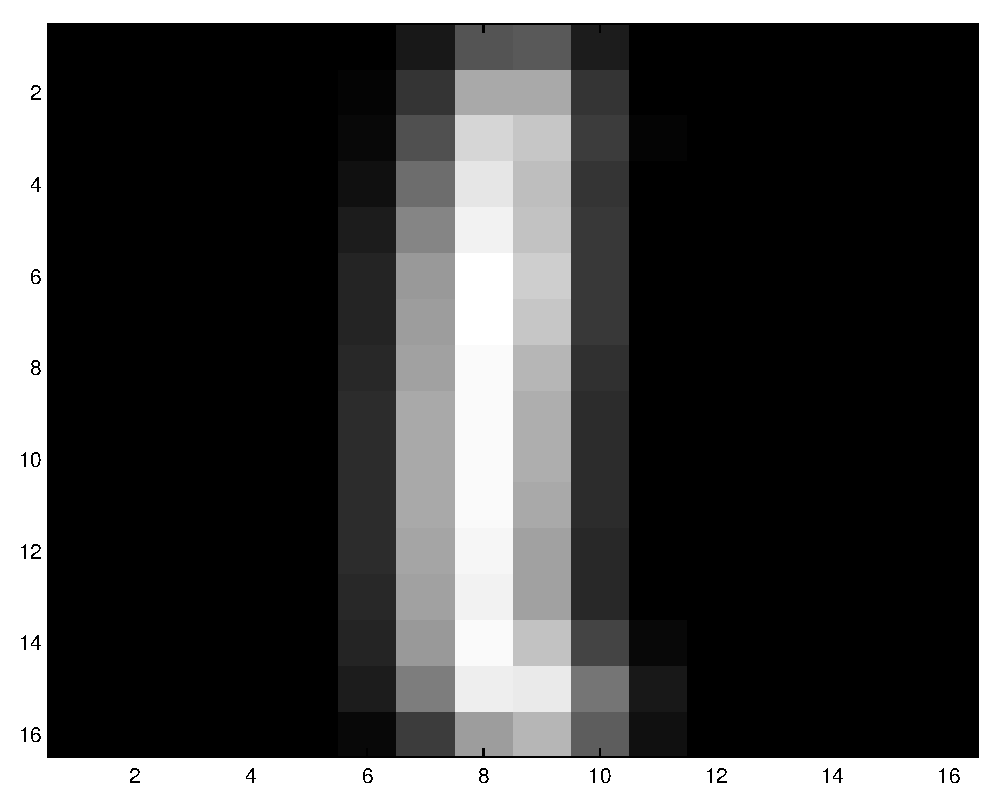
\includegraphics[width=0.25\textwidth]{digits3.eps}\hspace{0.03\textwidth}%
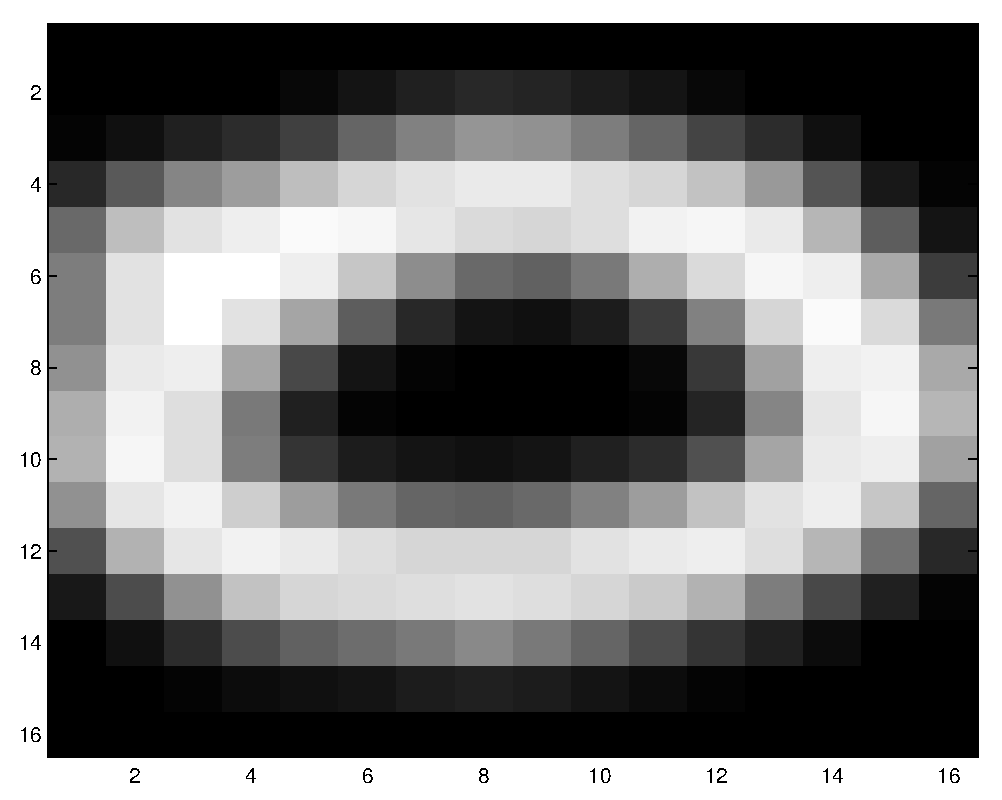
\includegraphics[width=0.25\textwidth]{digits4.eps}\\[1em]
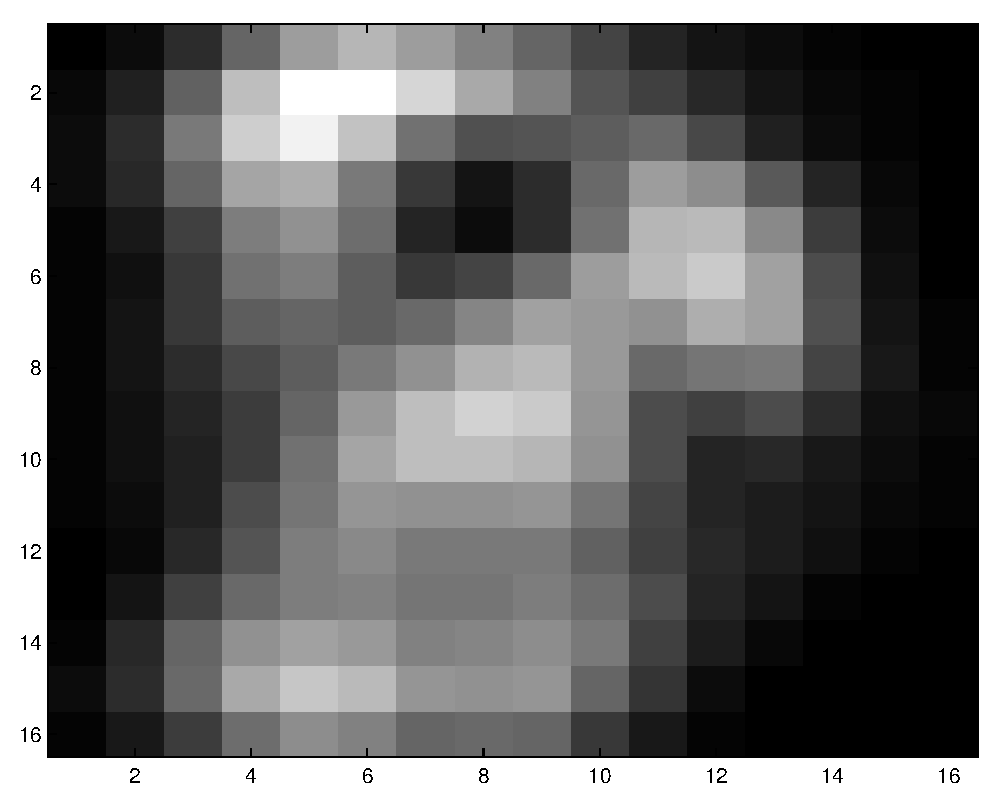
\includegraphics[width=0.25\textwidth]{reconst1.eps}\hspace{0.03\textwidth}%
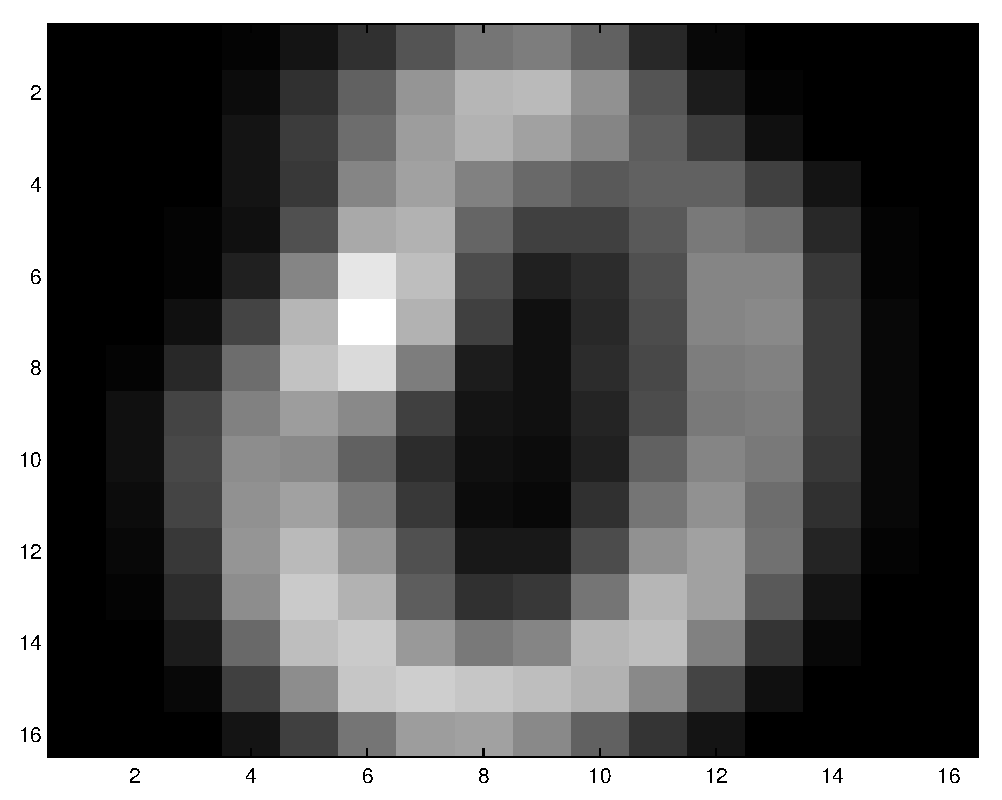
\includegraphics[width=0.25\textwidth]{reconst2.eps}\hspace{0.03\textwidth}%
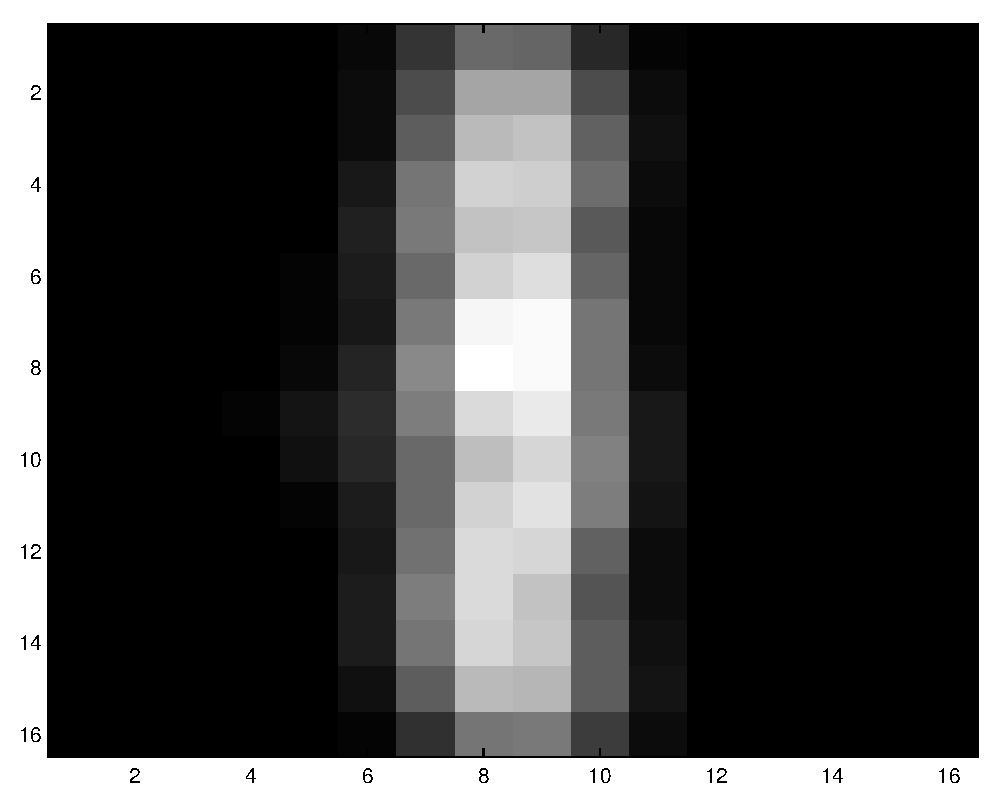
\includegraphics[width=0.25\textwidth]{reconst3.eps}\hspace{0.03\textwidth}%
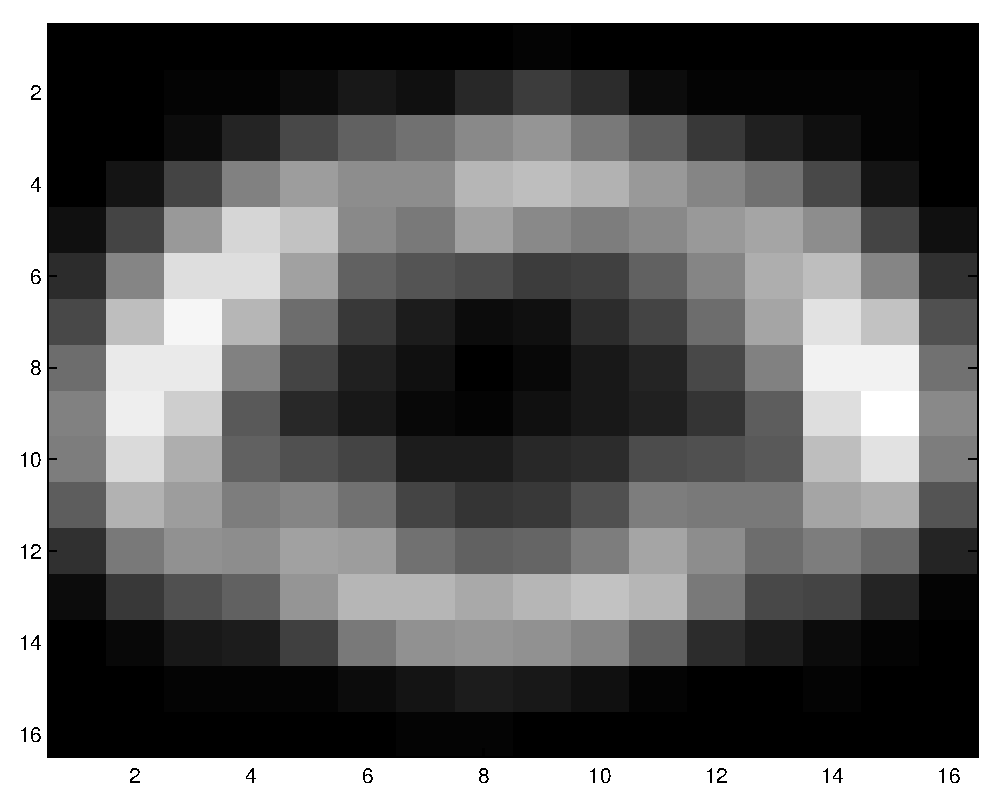
\includegraphics[width=0.25\textwidth]{reconst4.eps}\\[1em]
\rule{1.09\textwidth}{0.4pt}\\[1em]
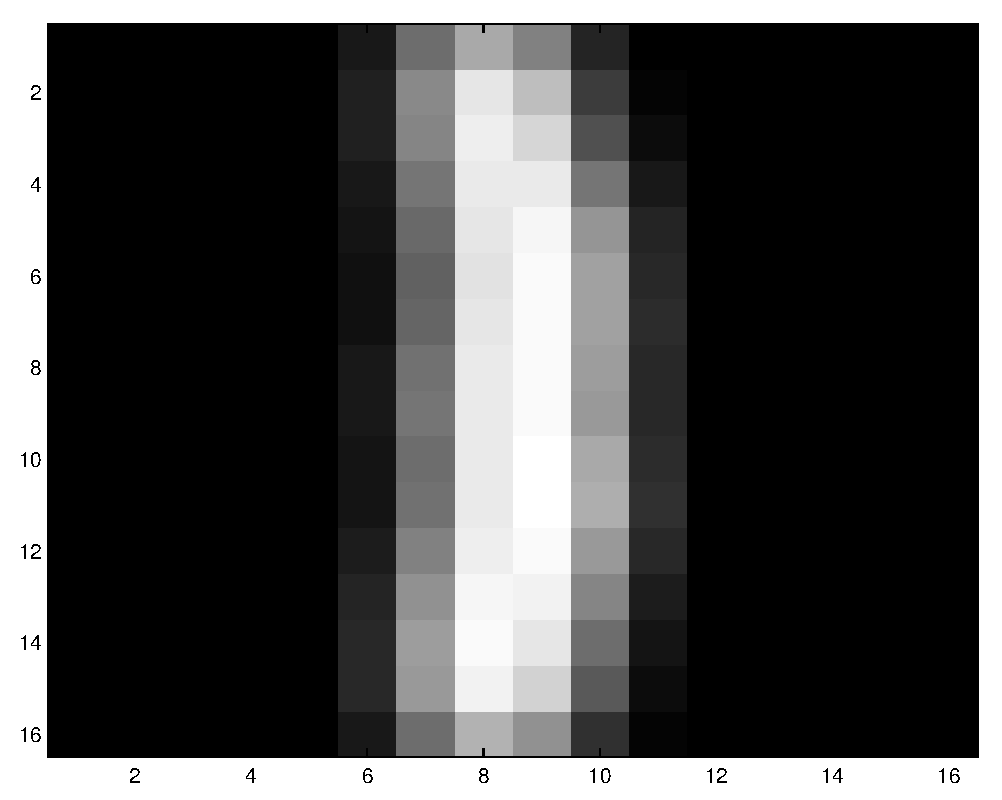
\includegraphics[width=0.25\textwidth]{digits5.eps}\hspace{0.03\textwidth}%
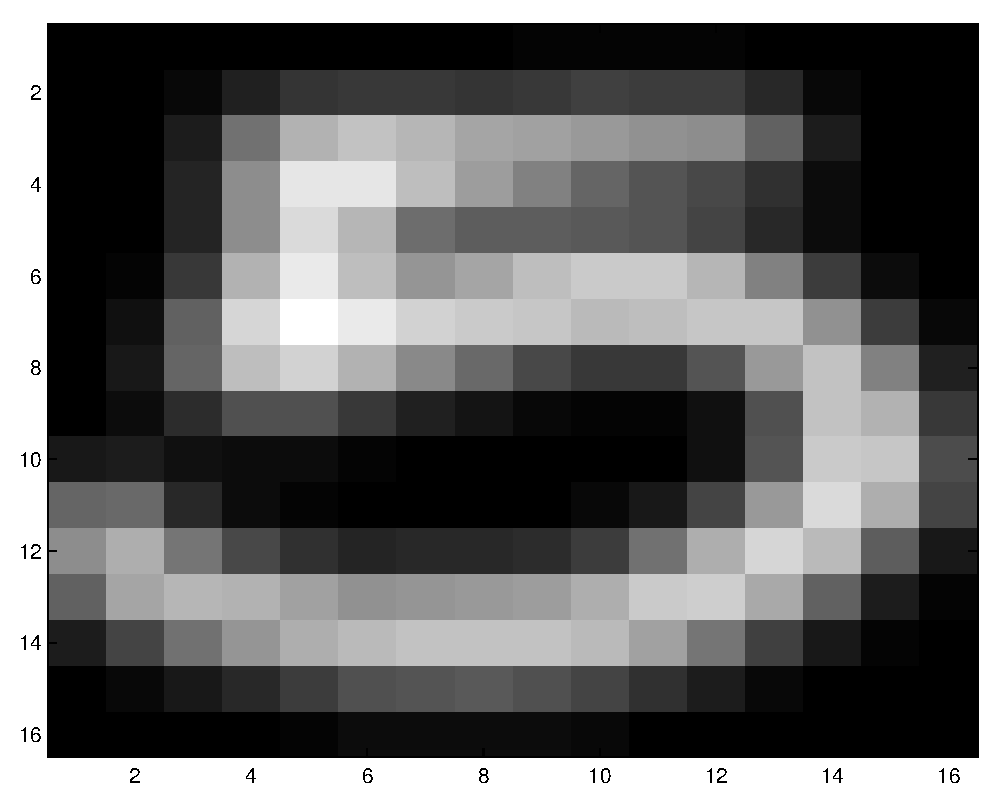
\includegraphics[width=0.25\textwidth]{digits6.eps}\hspace{0.03\textwidth}%
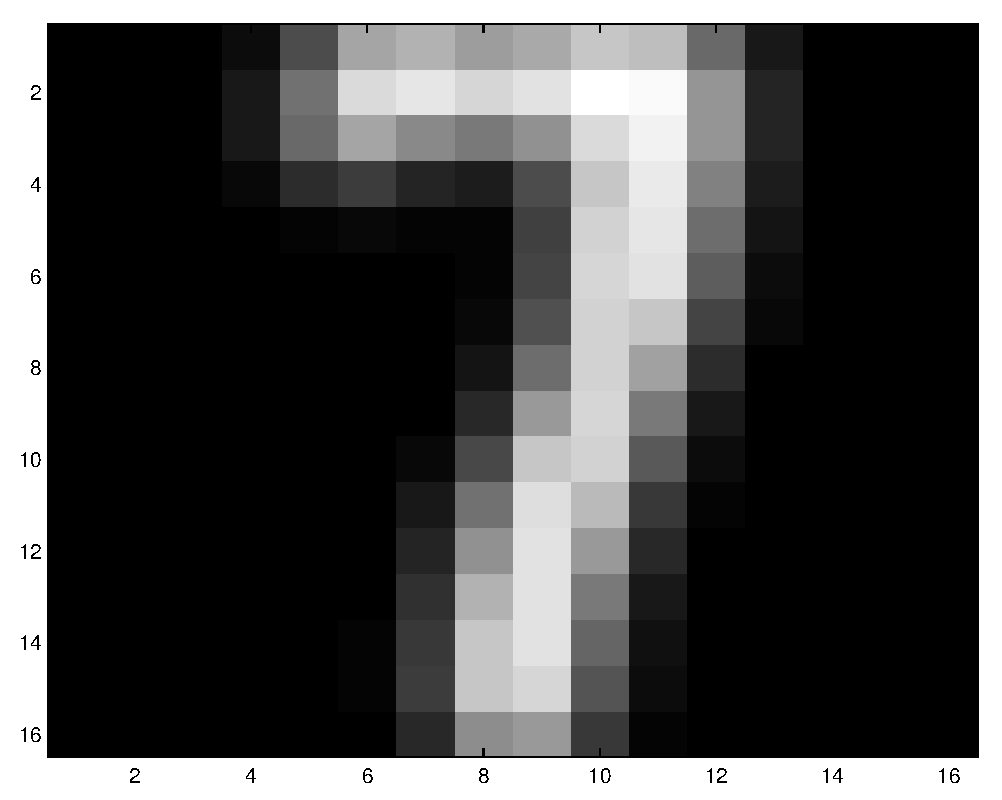
\includegraphics[width=0.25\textwidth]{digits7.eps}\hspace{0.03\textwidth}%
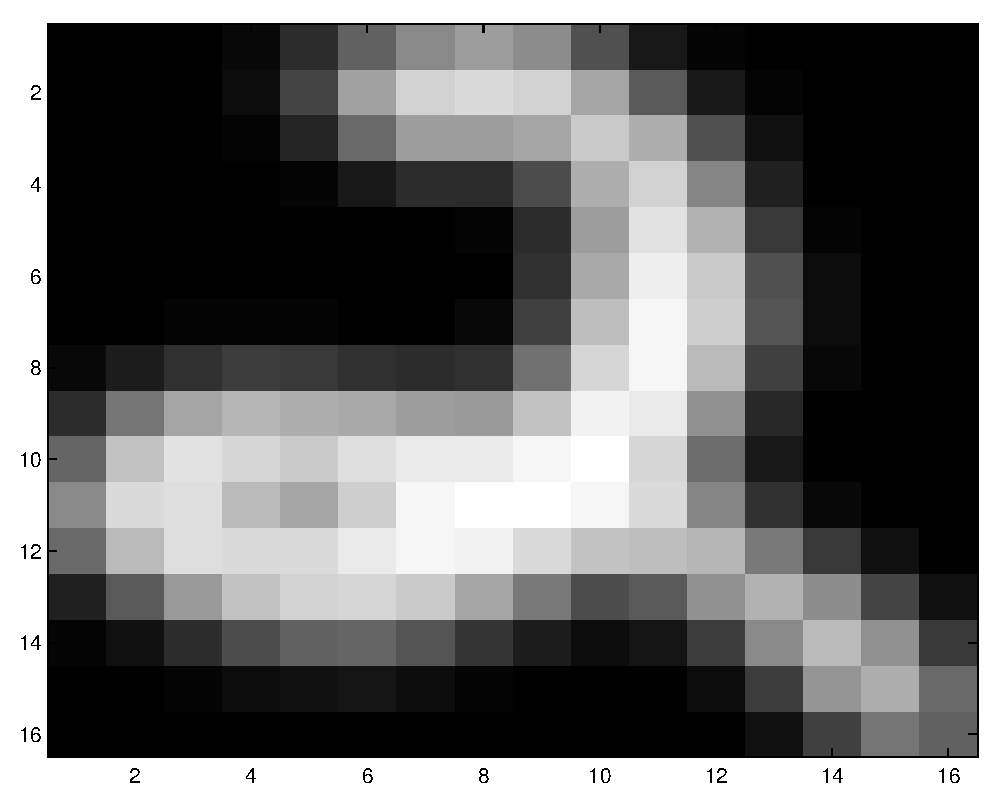
\includegraphics[width=0.25\textwidth]{digits8.eps}\\[1em]
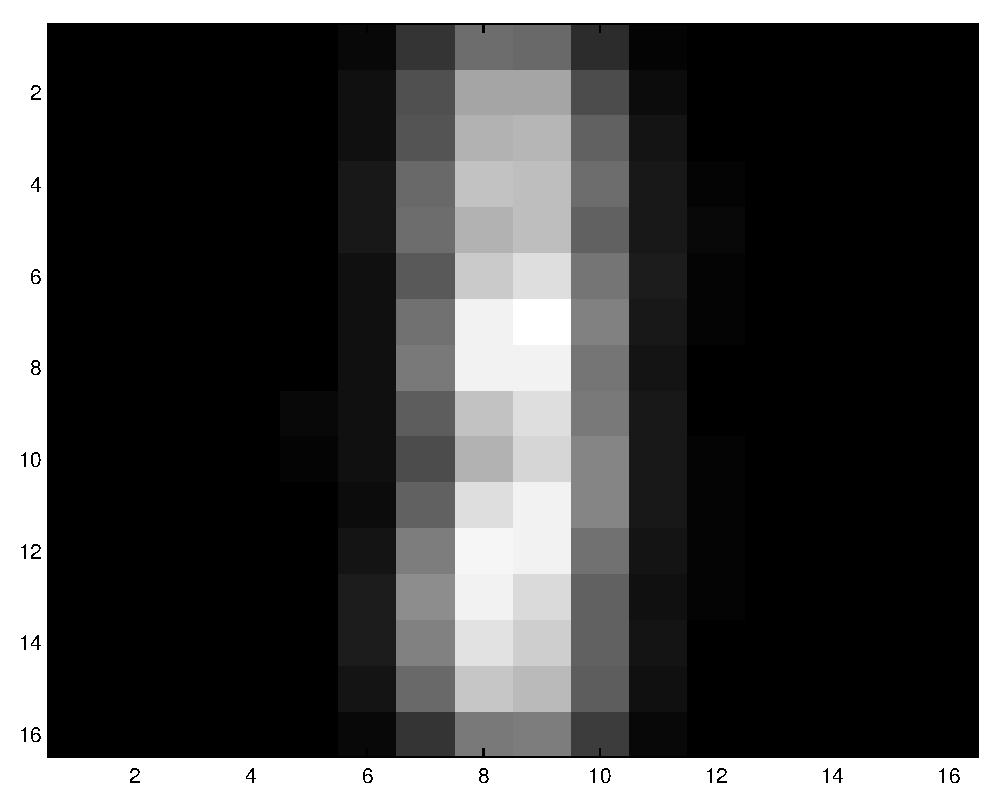
\includegraphics[width=0.25\textwidth]{reconst5.eps}\hspace{0.03\textwidth}%
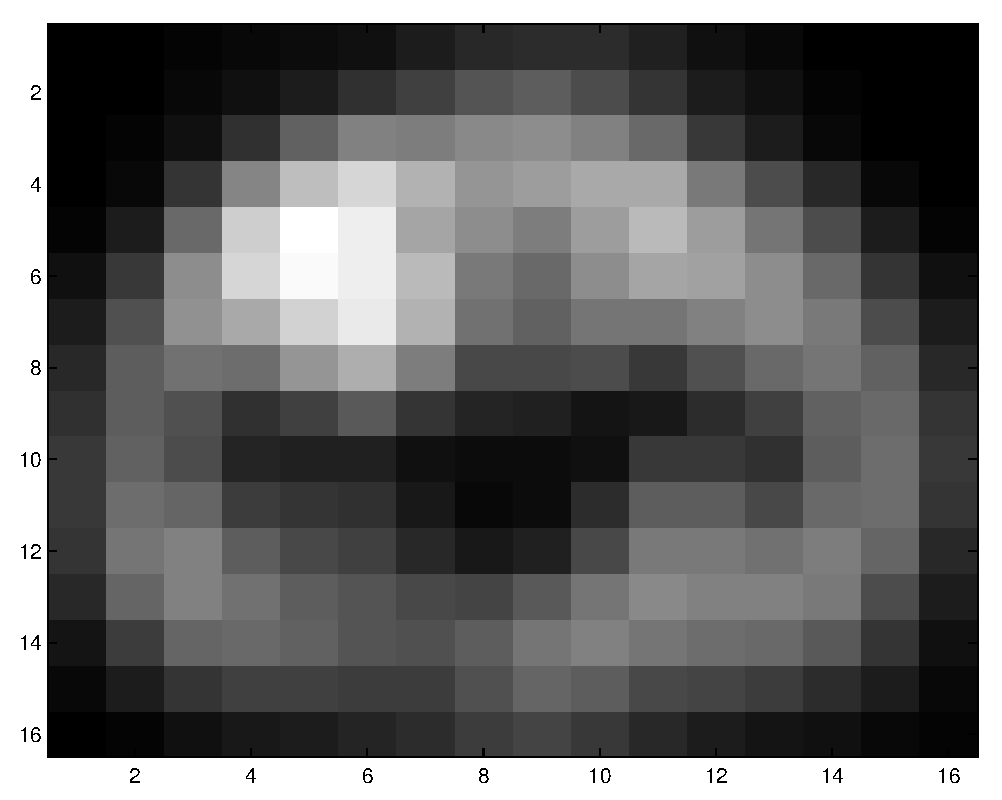
\includegraphics[width=0.25\textwidth]{reconst6.eps}\hspace{0.03\textwidth}%
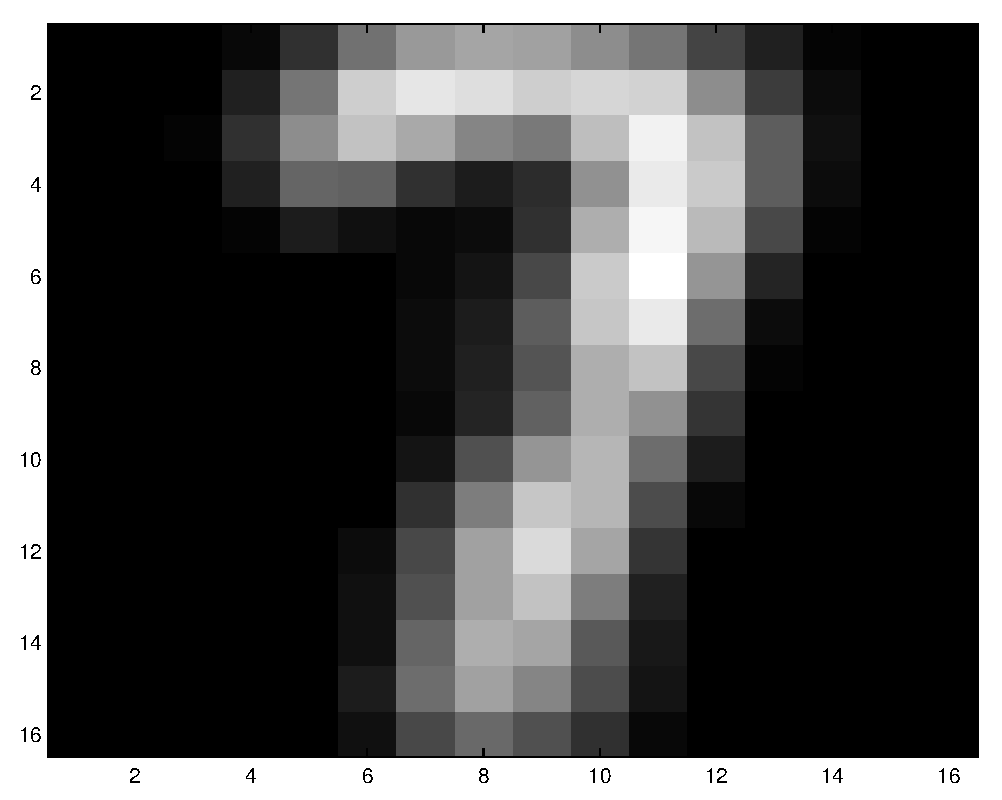
\includegraphics[width=0.25\textwidth]{reconst7.eps}\hspace{0.03\textwidth}%
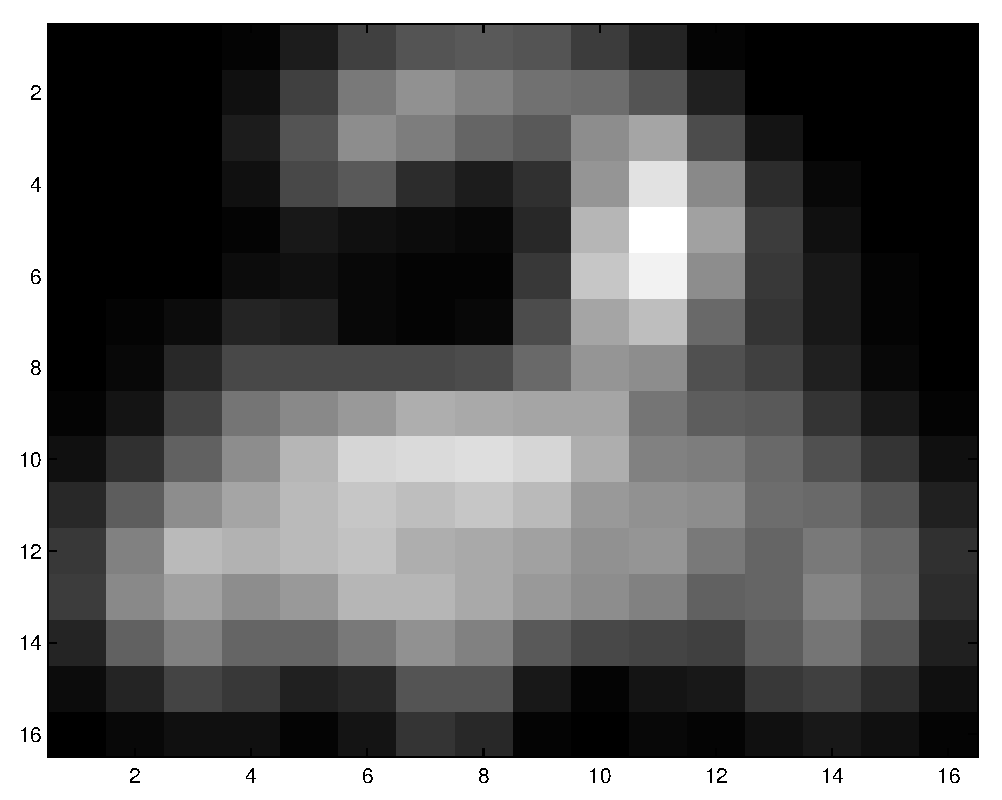
\includegraphics[width=0.25\textwidth]{reconst8.eps}\\[4em]
\newpage
\subsubsection*{Ein paar Bilder und deren Rekonstruktionen 300 Iterationen 50 Codewörter}
Im Folgenden sieht man in 2 Doppelreihen die ersten 8 Originalen
Bilder (jeweils oben) und die zugehörigen Rekonstruktionen (jeweils
unten). Insbesondere bei der Ziffer 5 sieht man, dass bei einem
größeren Codebook die Reproduktion optisch besser erkennbar ist. In
Aufgabe 2 stellen wir jedoch fest, dass sich das sehr geringfügig auf
die Erkennungsraten auswirkt.
\\
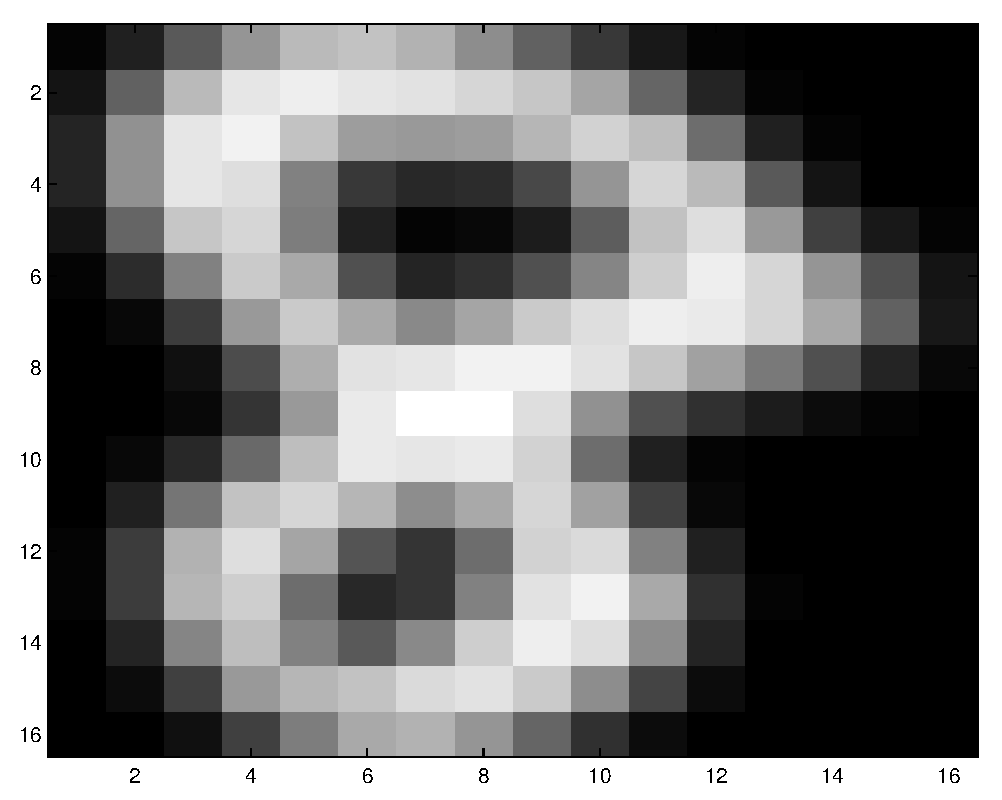
\includegraphics[width=0.25\textwidth]{50digits1.eps}\hspace{0.03\textwidth}%
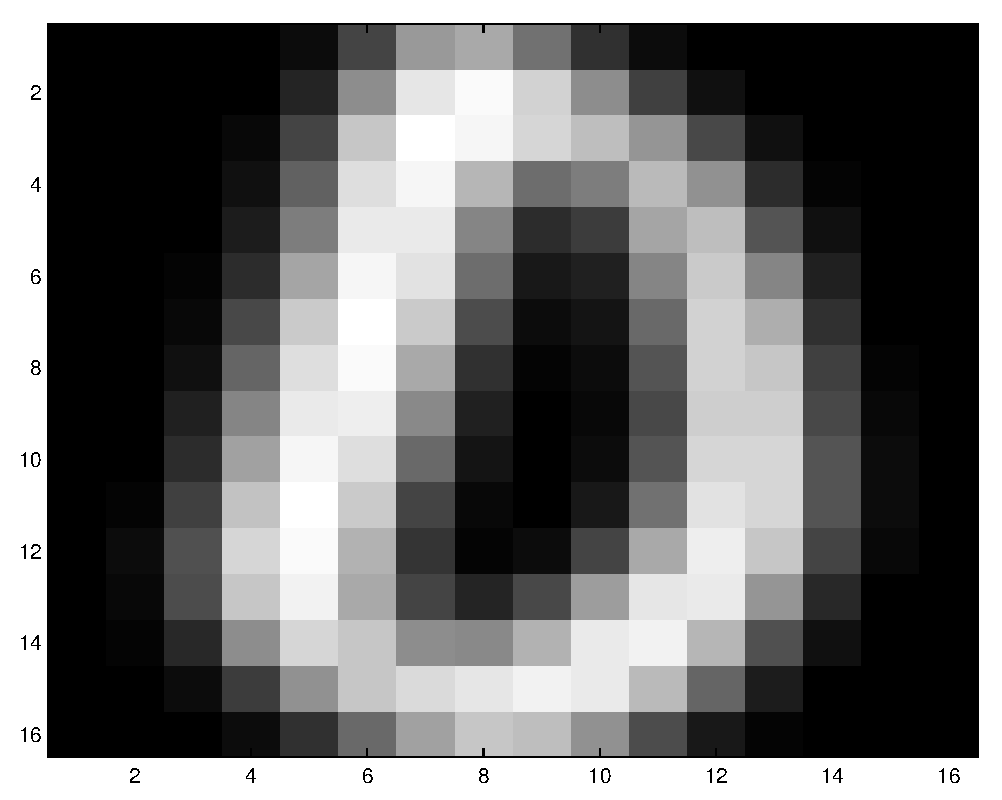
\includegraphics[width=0.25\textwidth]{50digits2.eps}\hspace{0.03\textwidth}%
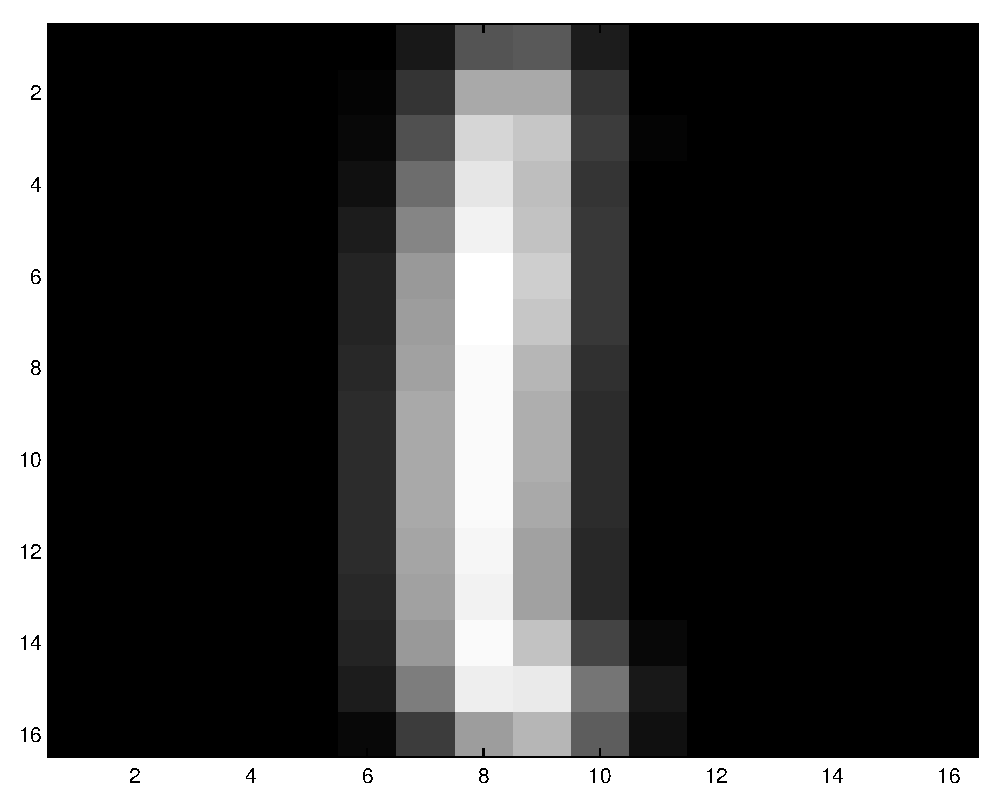
\includegraphics[width=0.25\textwidth]{50digits3.eps}\hspace{0.03\textwidth}%
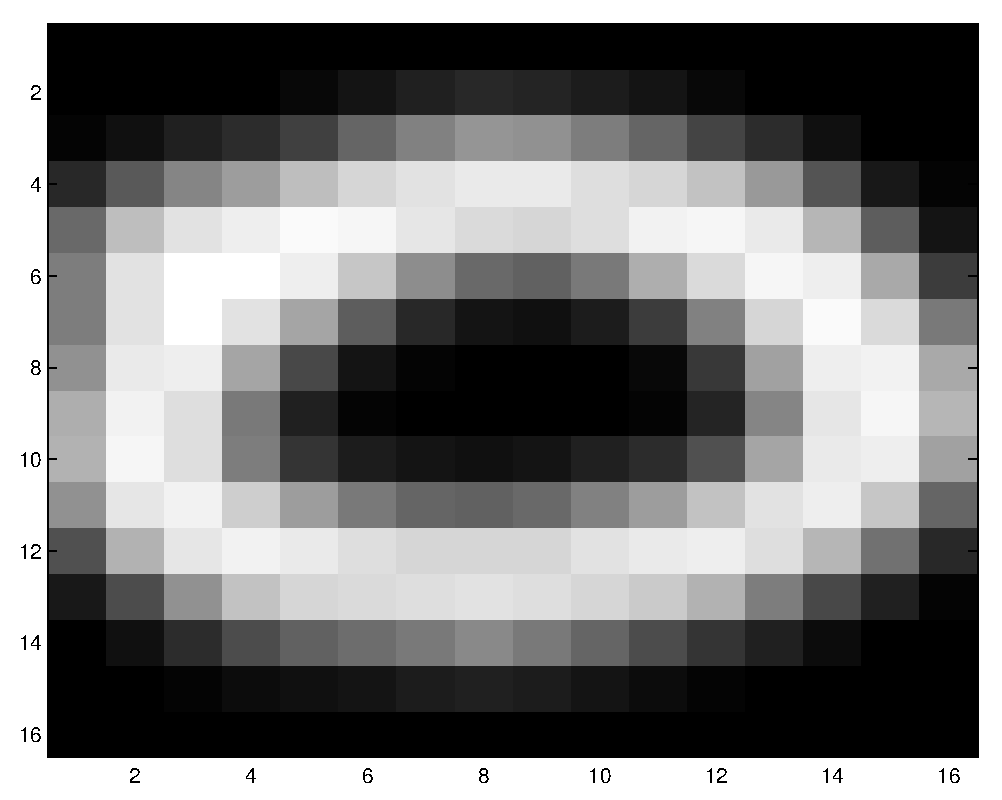
\includegraphics[width=0.25\textwidth]{50digits4.eps}\\[1em]
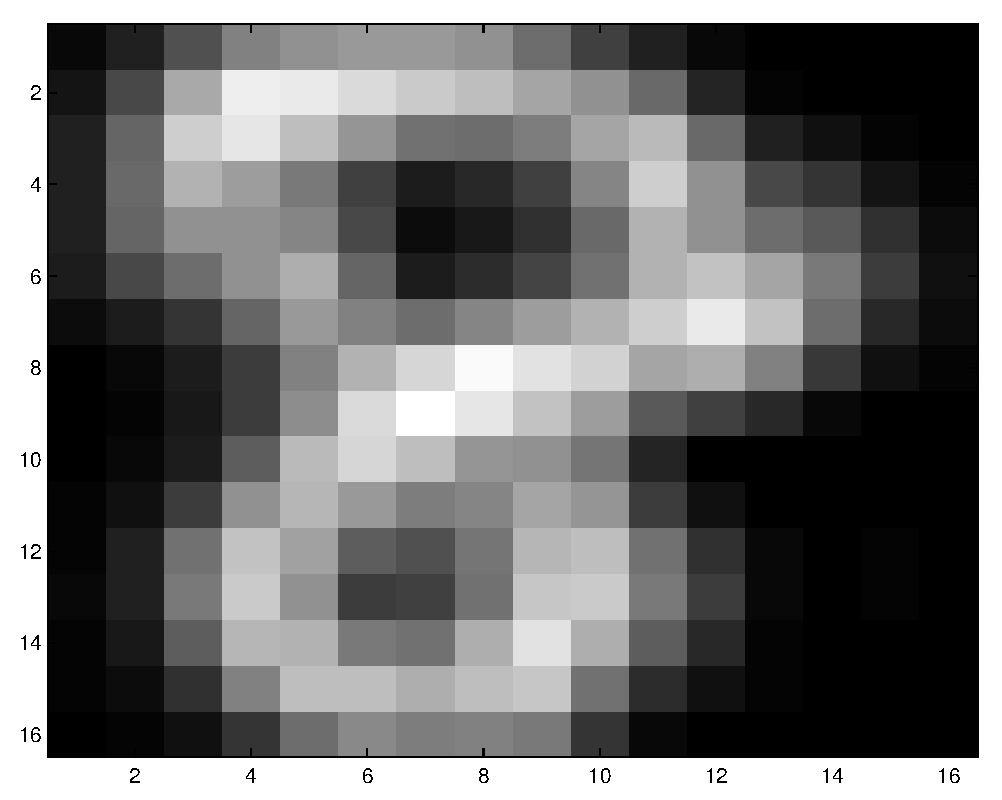
\includegraphics[width=0.25\textwidth]{50reconst1.eps}\hspace{0.03\textwidth}%
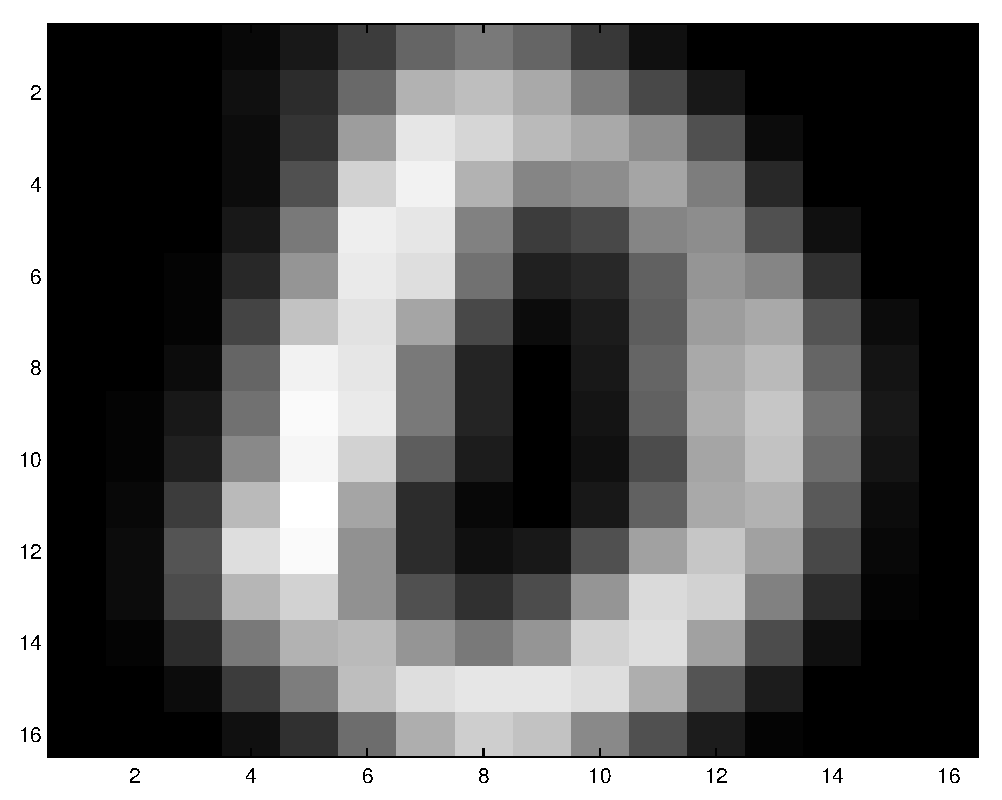
\includegraphics[width=0.25\textwidth]{50reconst2.eps}\hspace{0.03\textwidth}%
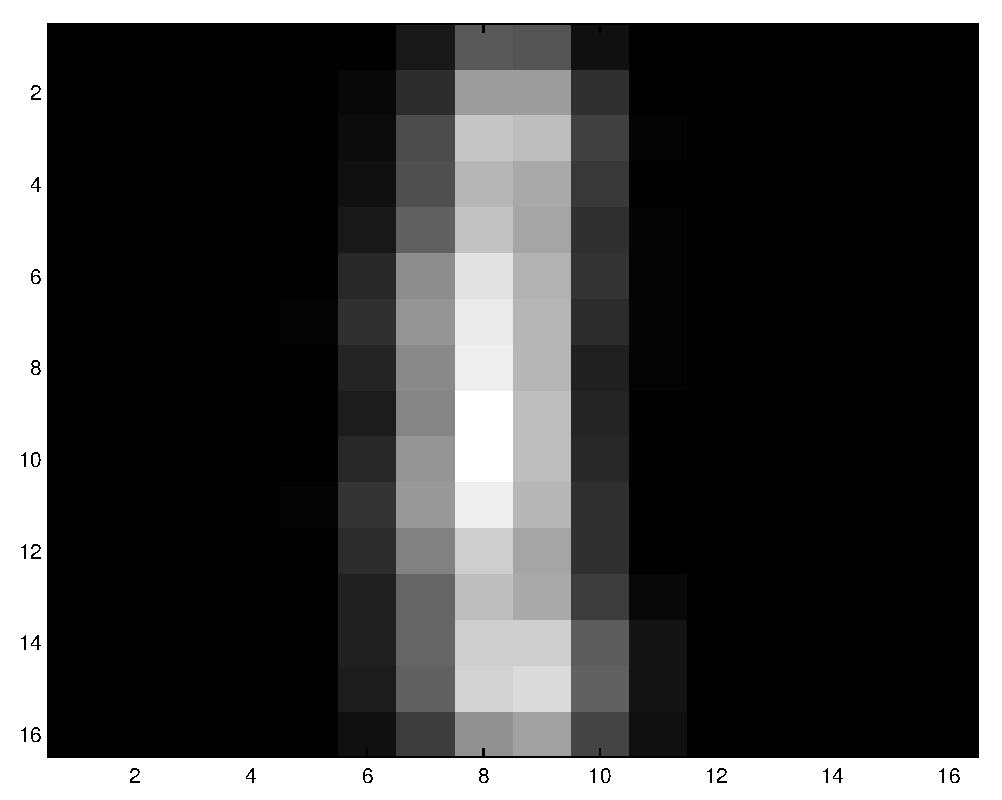
\includegraphics[width=0.25\textwidth]{50reconst3.eps}\hspace{0.03\textwidth}%
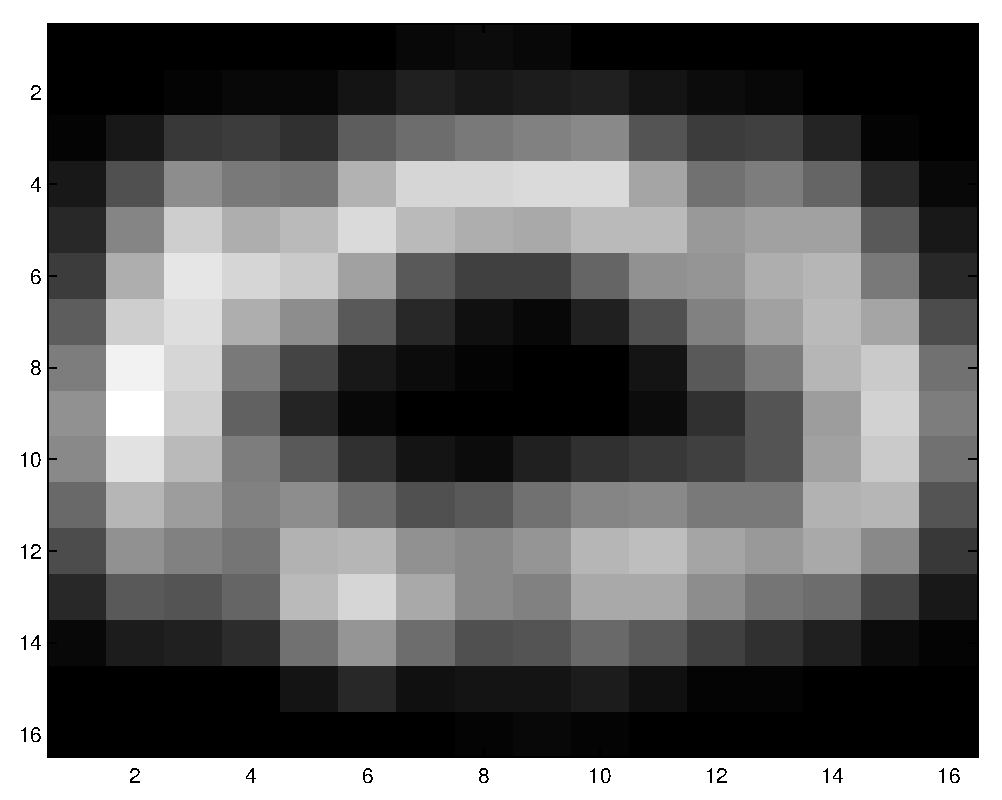
\includegraphics[width=0.25\textwidth]{50reconst4.eps}\\[1em]
\rule{1.09\textwidth}{0.4pt}\\[1em]
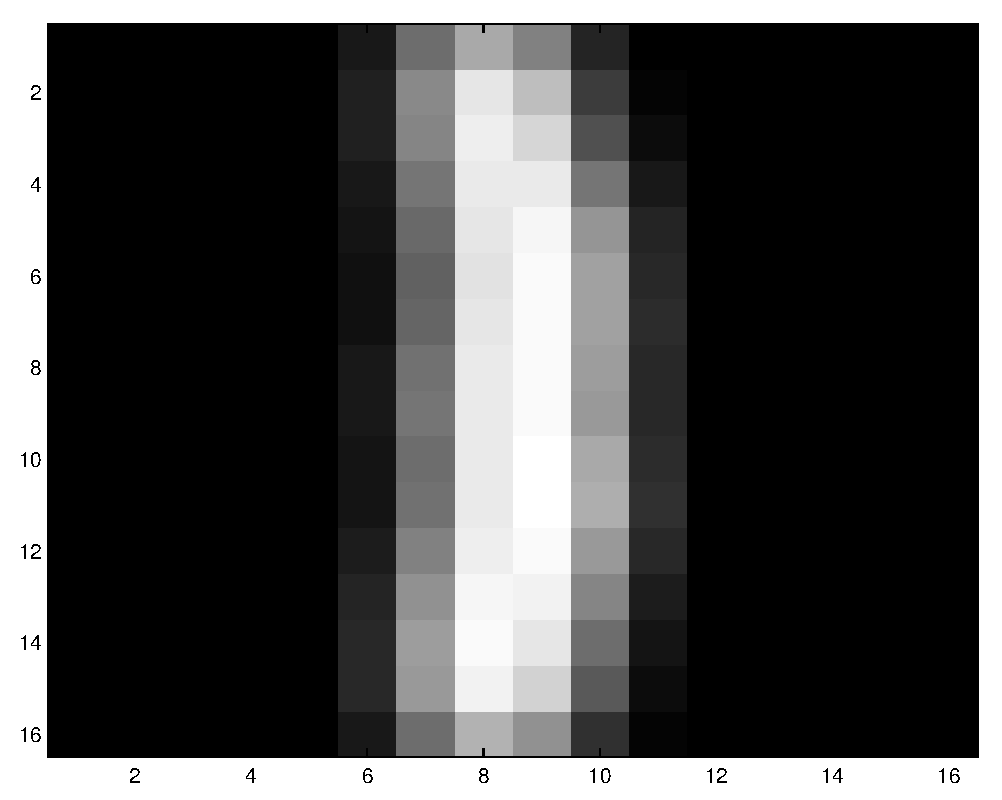
\includegraphics[width=0.25\textwidth]{50digits5.eps}\hspace{0.03\textwidth}%
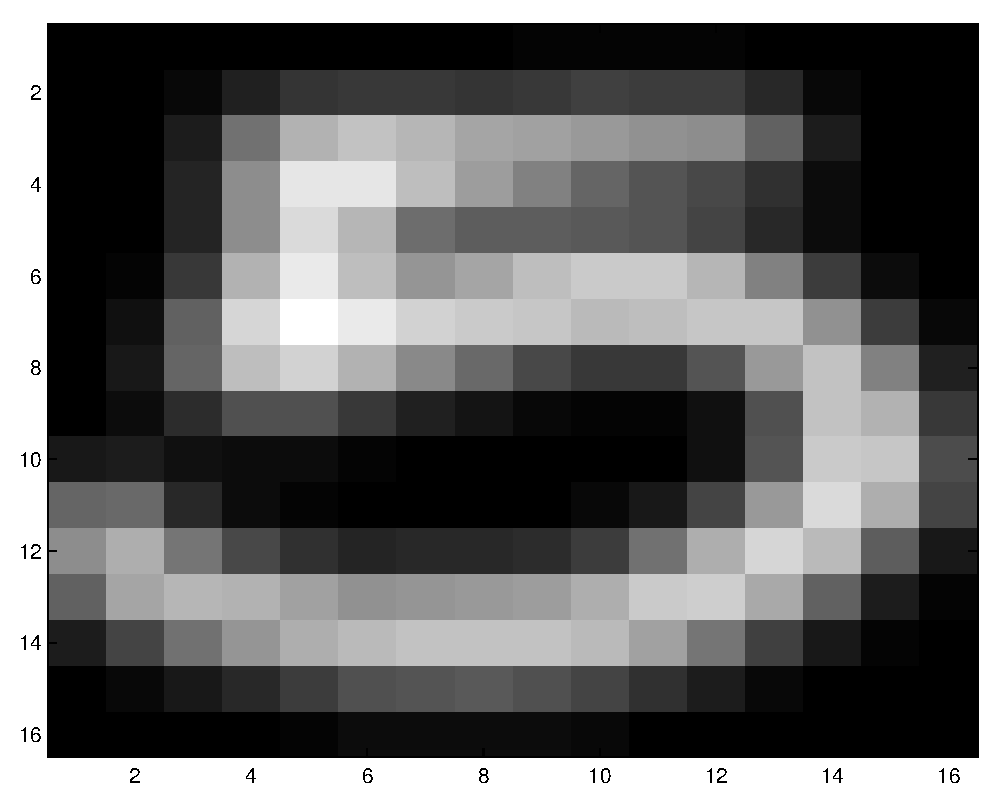
\includegraphics[width=0.25\textwidth]{50digits6.eps}\hspace{0.03\textwidth}%
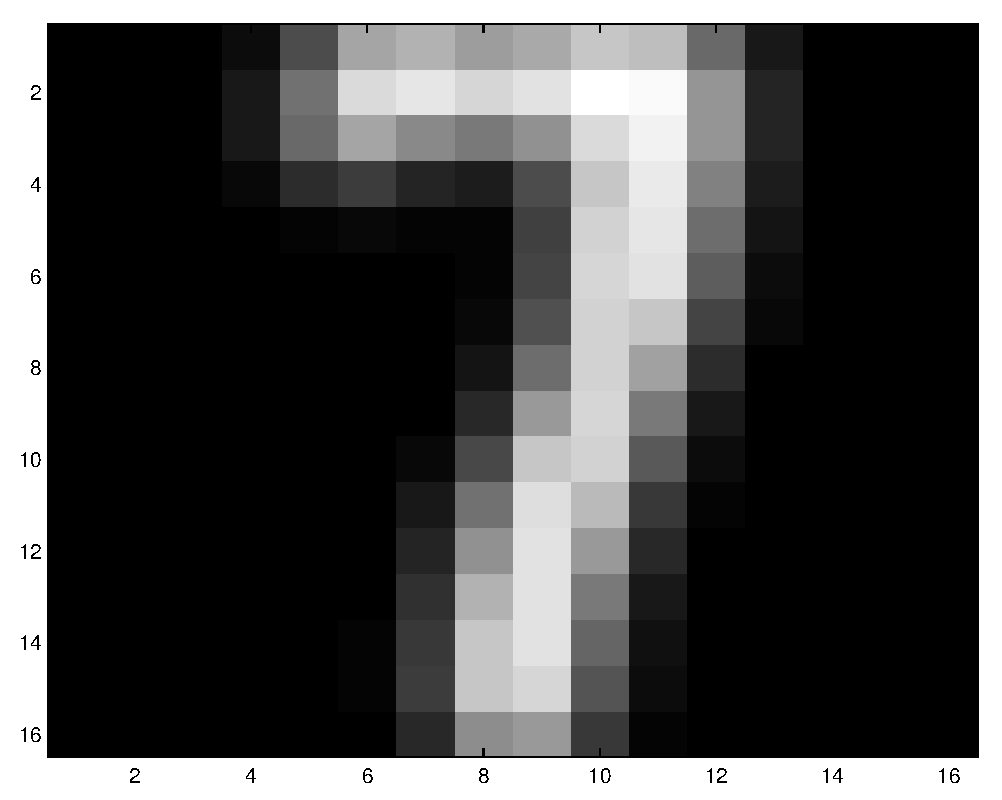
\includegraphics[width=0.25\textwidth]{50digits7.eps}\hspace{0.03\textwidth}%
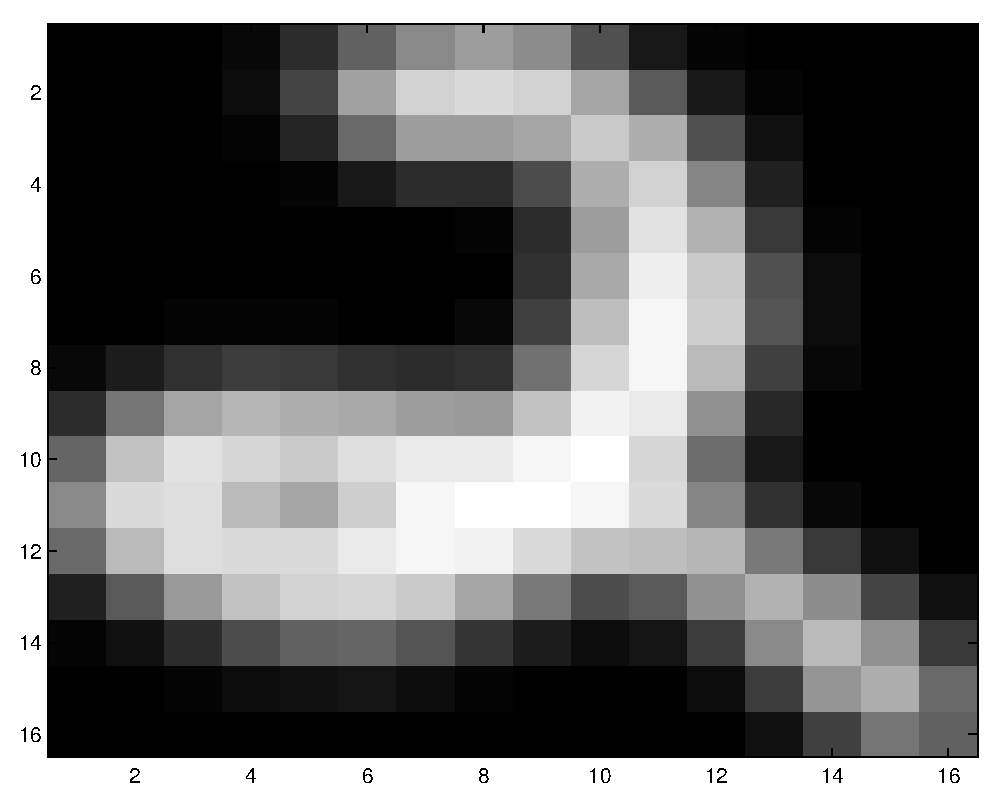
\includegraphics[width=0.25\textwidth]{50digits8.eps}\\[1em]
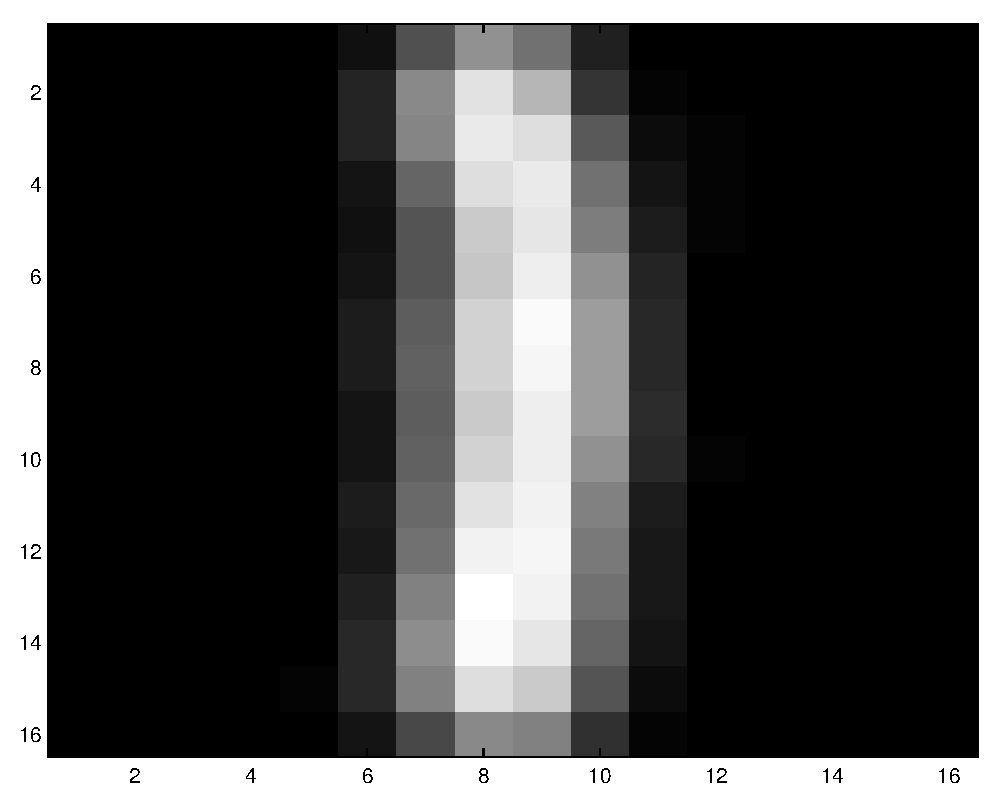
\includegraphics[width=0.25\textwidth]{50reconst5.eps}\hspace{0.03\textwidth}%
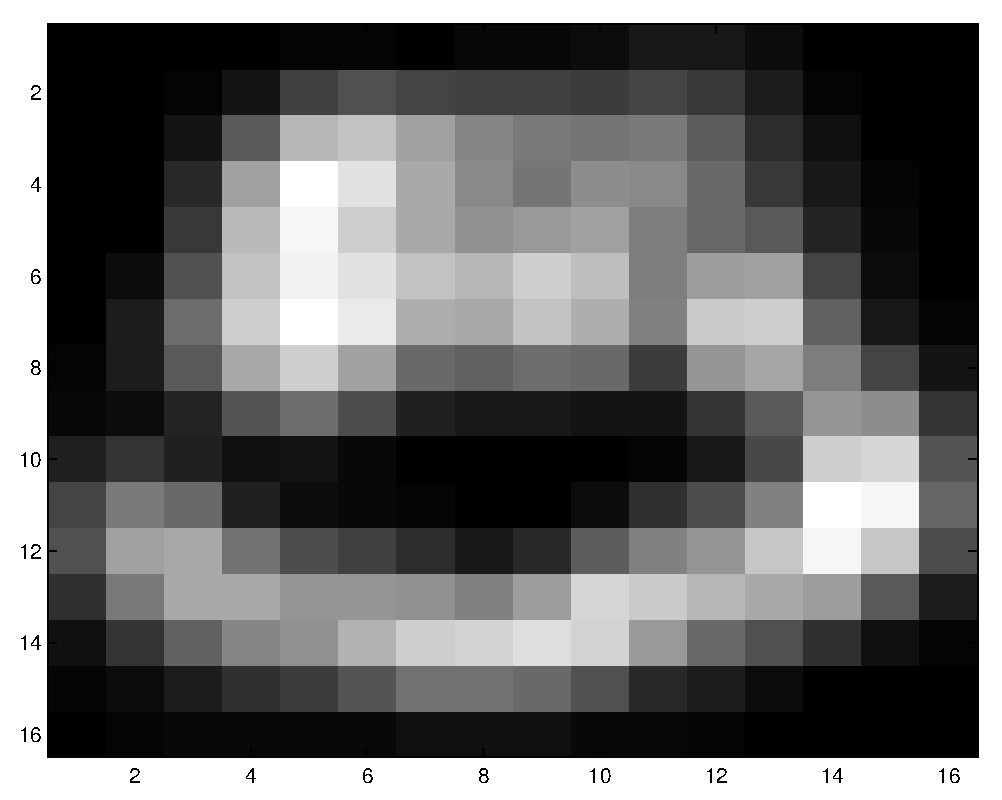
\includegraphics[width=0.25\textwidth]{50reconst6.eps}\hspace{0.03\textwidth}%
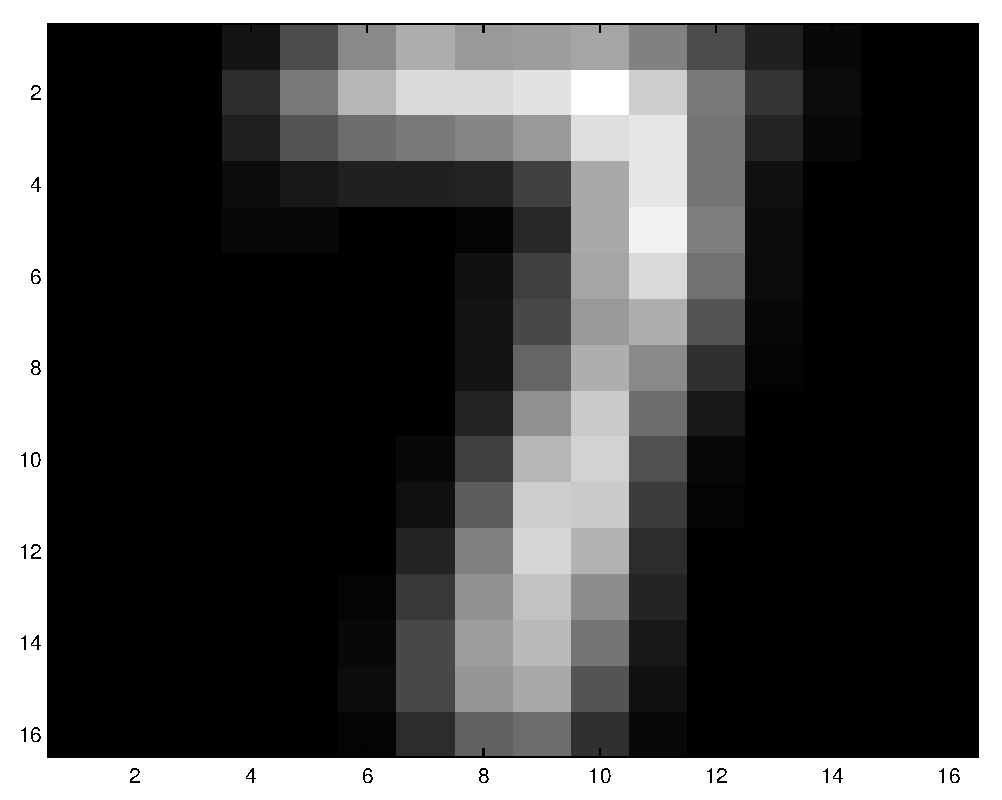
\includegraphics[width=0.25\textwidth]{50reconst7.eps}\hspace{0.03\textwidth}%
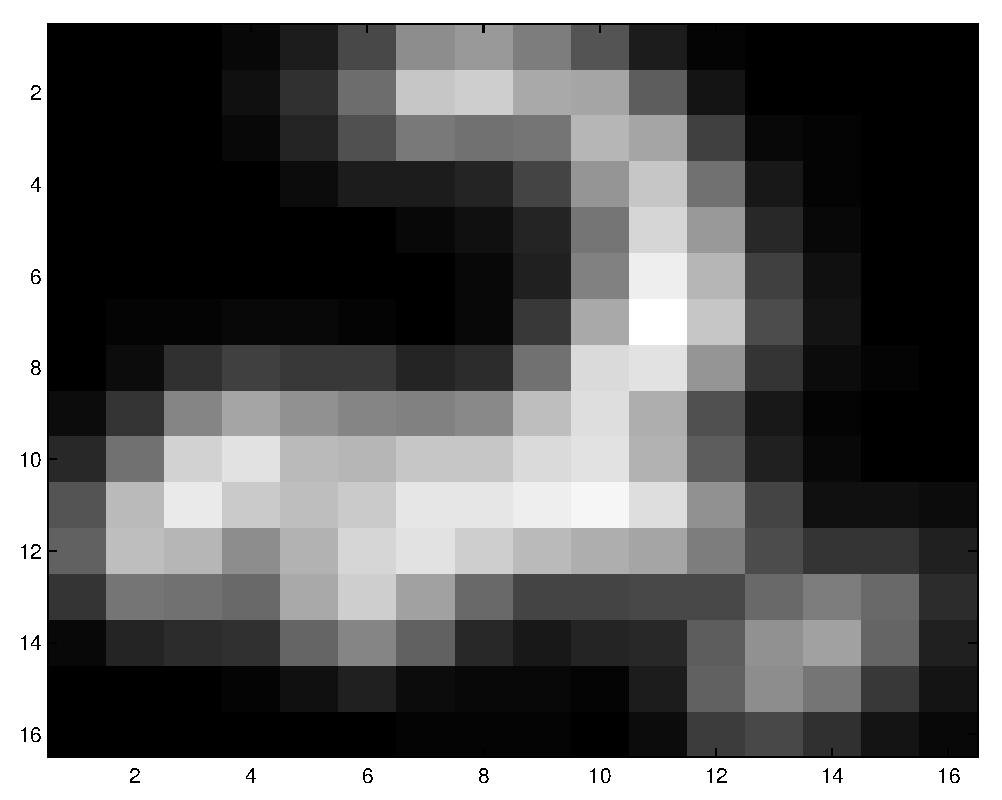
\includegraphics[width=0.25\textwidth]{50reconst8.eps}\\[4em]
\newpage
\subsection*{2. Auswertung}
Wir haben die Erkennungsraten mit NMF, PCA und ohne Vorverarbeitung
mit folgendem Code verglichen. Eine effiziente kNearestNeighbors
Funktion haben wir dem Internet entnommen. Das ergebnis war wie folgt (k=3):\\
\begin{tabular}{ l |c }
  & Erkennungrate\\
  \hline
  NMF (32 Codewörter) & 94.51\% \\
  NMF (20 Codewörter) & 94.51\% \\
  NMF (4 Codewörter) & 60.74\% \\
  PCA (100 Dimensionen) & 96.86\% \\
  PCA (60 Dimensionen) & 96.88\% \\
  PCA (30 Dimensionen) & 96.82\% \\
  PLAIN & 96.86\% \\
  \hline
\end{tabular}\\
Unsere Tests haben ergeben, dass 20 eine gute Größe für ein Codebuch ist.
\begin{lstlisting}
function compute_knn
  tra_p = load('usps.ascii/train_patterns.txt'); 
  tra_l = load('usps.ascii/train_labels.txt');
  tes_p = load('usps.ascii/test_patterns.txt');
  tes_l = load('usps.ascii/test_labels.txt');


  [neighbors distances] = kNearestNeighbors(tra_p', tes_p', 3)
  save('plain_neighbors3.mat','neighbors');

  % pca
  traX = tra_p';
  traY = dummyToNumber(tra_l');
  tesX = tes_p';
  tesY = dummyToNumber(tes_l');

  pcaBase = pca_get_base(traX);
  traX_t = pca_transform(pcaBase, traX, 60);  % Original has 256
  tesX_t = pca_transform(pcaBase, tesX, 60);  % Original has 256

  [neighbors distances] = kNearestNeighbors(traX_t, tesX_t, 3);
  save('pca_neighbors3.mat','neighbors');

  % nmf
  W = load('w1000_32.mat'); W = W.W;
  H = load('h1000_32.mat'); H = H.H;
  
  H_tes = ((W'*W)^-1)*W'*tes_p;
  [neighbors distances] = kNearestNeighbors(H', H_tes', 3);
  save('nmf_neighbors3.mat','neighbors');
end

function numbers = dummyToNumber(dummies)
  [value index] = max(dummies, [], 2);
  numbers = index - 1;
end

function run_nmf(iterations)
  tra_p = load('usps.ascii/train_patterns.txt'); 
  
  sizes = [40 60 80];
  Ws = cell(8,1);
  Hs = cell(8,1);

  parfor i = 1:3
    [W H] = nmf(tra_p, sizes(i), iterations);
    Ws{i}(:,:) = W;
    Hs{i}(:,:) = H;
  end
  
  for i = 1:3
    num = sprintf('%d',sizes(i));
    its = sprintf('%d',iterations);
    W = Ws{i}(:,:);
    H = Hs{i}(:,:);
    nw = ['w' its '_' num '.mat']
    nh = ['h' its '_' num '.mat']
    save(nw,'W');
    save(nh,'H');
  end  
end

function test_results
  tra_p = load('usps.ascii/train_patterns.txt'); 
  tes_p = load('usps.ascii/test_patterns.txt');

  tra_l = load('usps.ascii/train_labels.txt');
  [val tra_l] = max(tra_l);
  tra_l = tra_l-1;

  tes_l = load('usps.ascii/test_labels.txt');
  [val tes_l] = max(tes_l);
  tes_l = tes_l-1;

  p = predict(tra_l, 'nmf_neighbors3.mat');
  isVsShould = [p' tes_l'];
  diff = isVsShould(:,1) - isVsShould(:,2);
  right = size(diff(diff==0));
  NmfSuccessRate = right /size(diff)

  p = predict(tra_l, 'plain_neighbors3.mat');
  isVsShould = [p' tes_l'];
  diff = isVsShould(:,1) - isVsShould(:,2);
  right = size(diff(diff==0));
  PlainSuccessRate = right /size(diff)

  p = predict(tra_l, 'pca_neighbors3.mat');
  isVsShould = [p' tes_l'];
  diff = isVsShould(:,1) - isVsShould(:,2);
  right = size(diff(diff==0));
  PcaSuccessRate = right /size(diff)
end

function r = predict(tra_l,filename)
  results = load(filename,'neighbors');
  results = results.neighbors;
  r = mode(tra_l(results)');
end
\end{lstlisting}

\newpage
\subsection*{3. Das Codebuch}
Im Folgenden ist ein Codebuch mit 20 Codewörtern nach 1000 Iterationen
dargestellt:\\
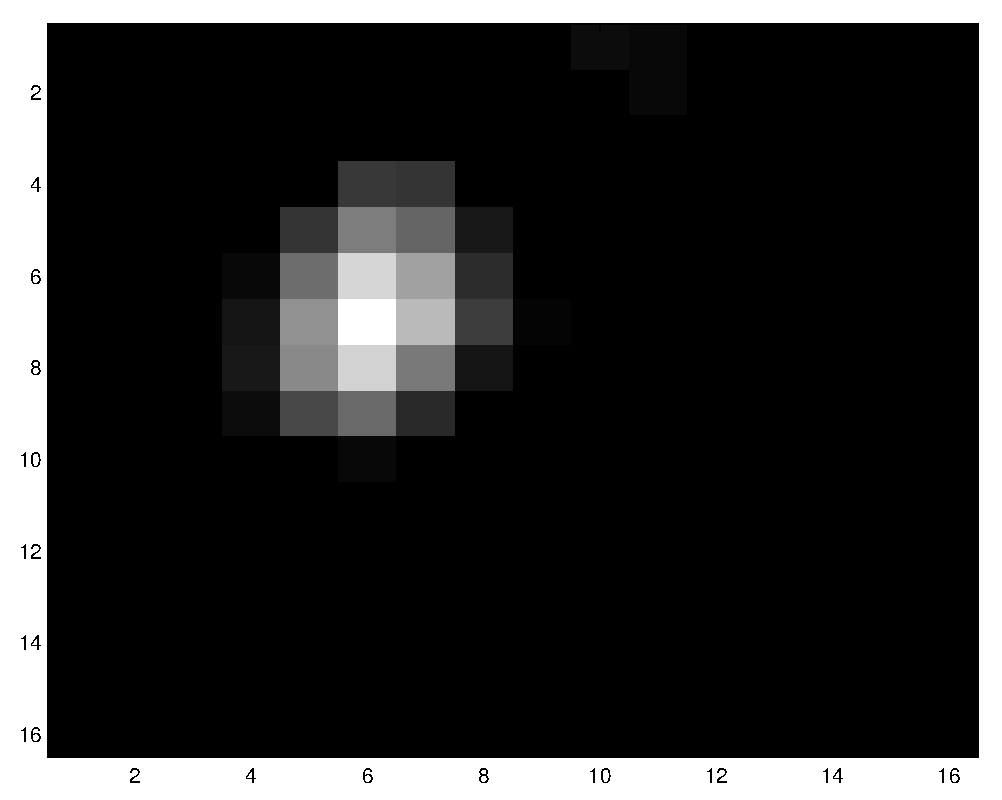
\includegraphics[width=0.25\textwidth]{codebook1.eps}\hspace{0.03\textwidth}%
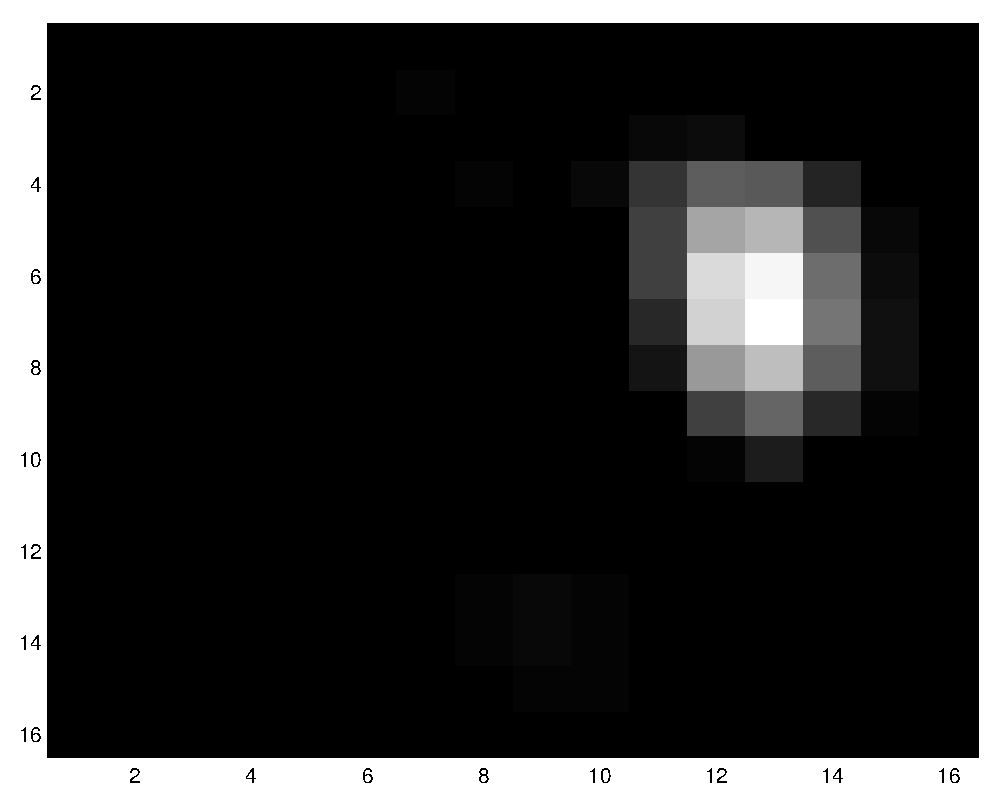
\includegraphics[width=0.25\textwidth]{codebook2.eps}\hspace{0.03\textwidth}%
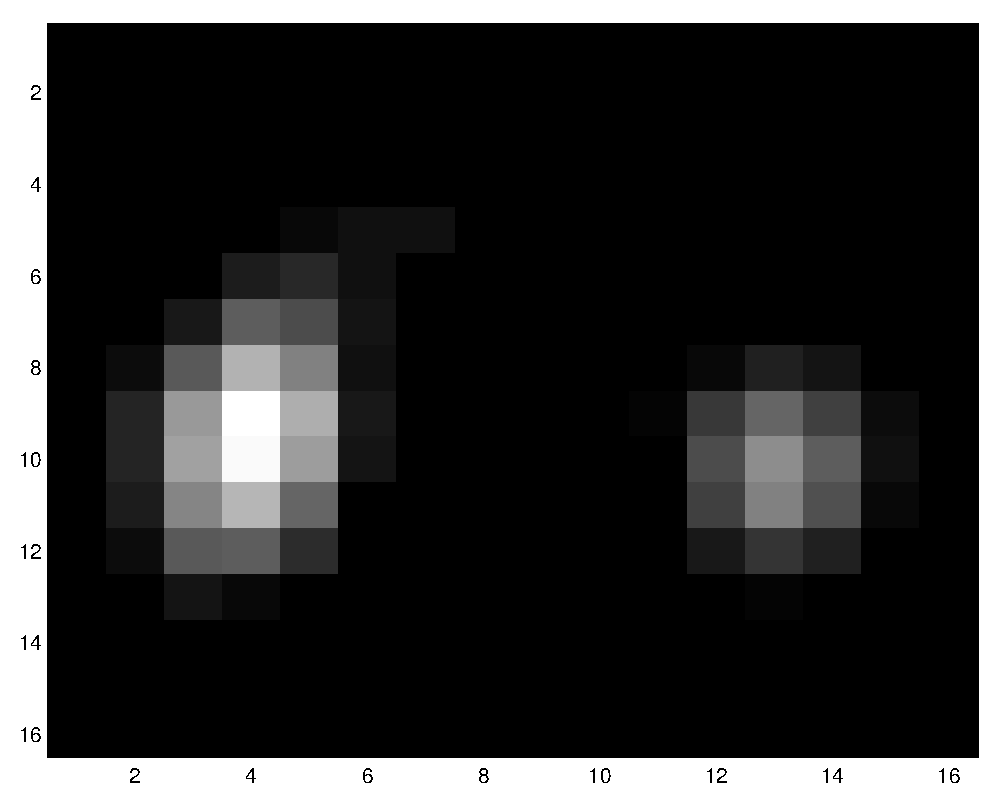
\includegraphics[width=0.25\textwidth]{codebook3.eps}\hspace{0.03\textwidth}%
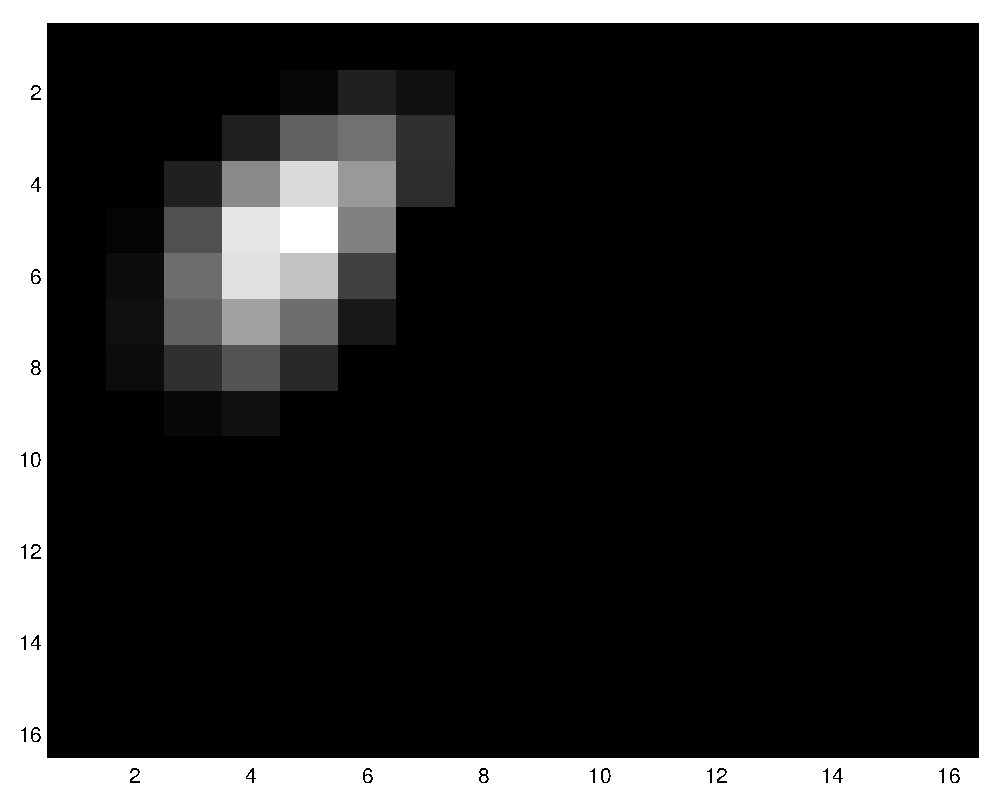
\includegraphics[width=0.25\textwidth]{codebook4.eps}\\[1em]
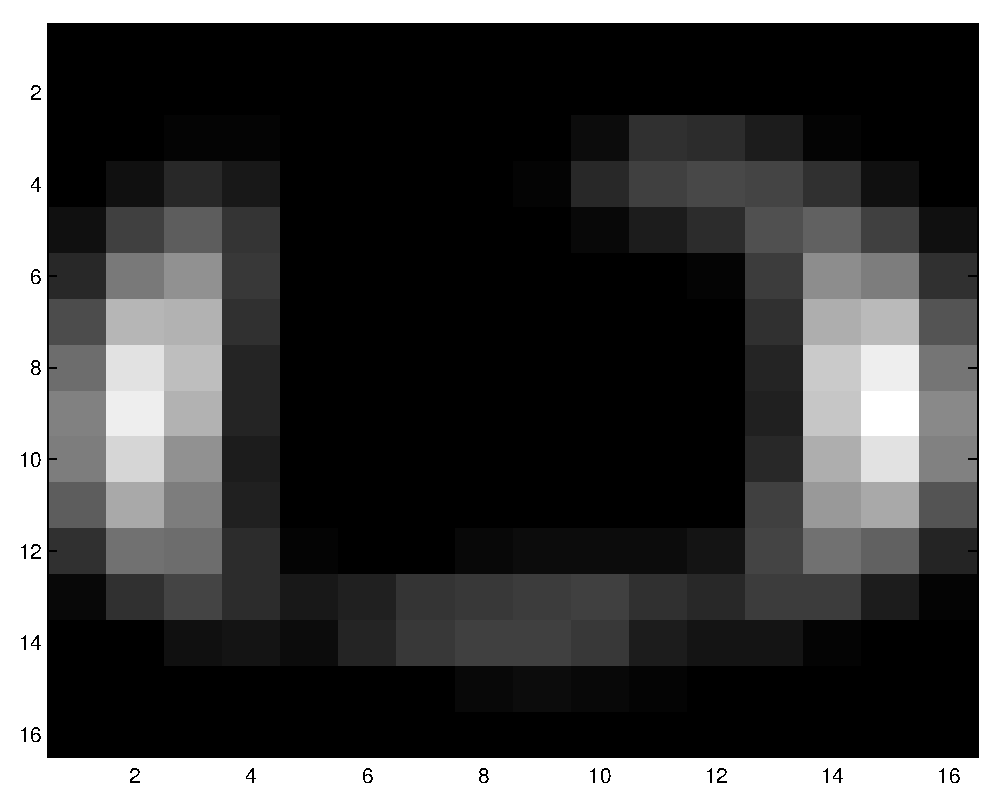
\includegraphics[width=0.25\textwidth]{codebook5.eps}\hspace{0.03\textwidth}%
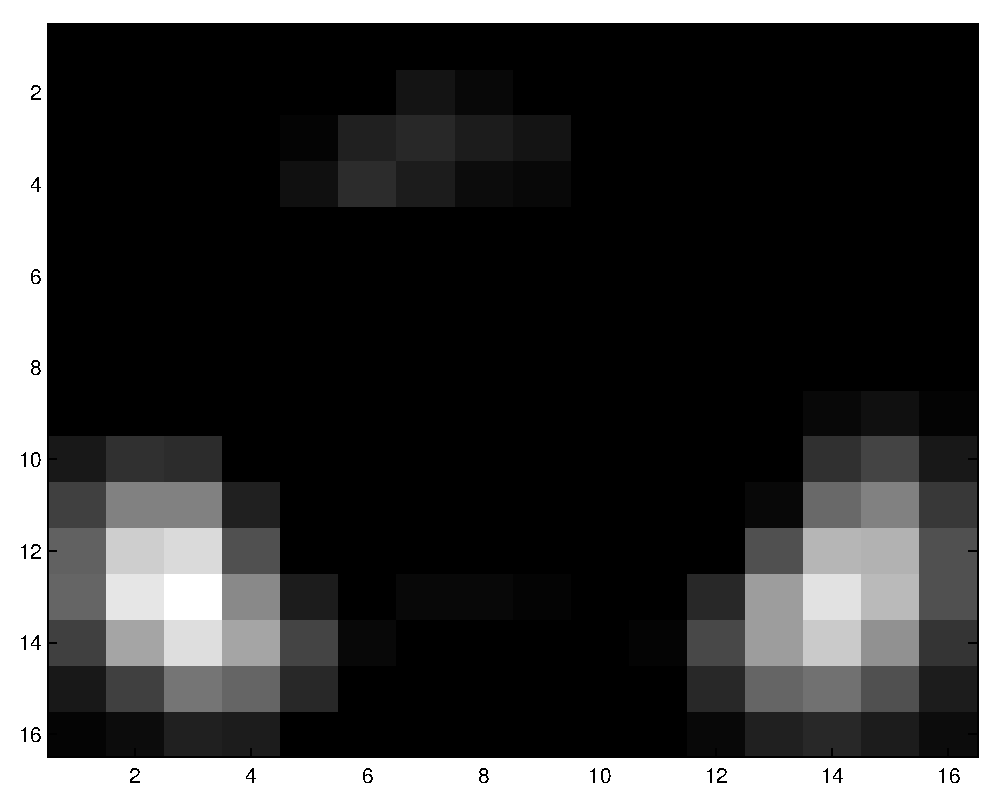
\includegraphics[width=0.25\textwidth]{codebook6.eps}\hspace{0.03\textwidth}%
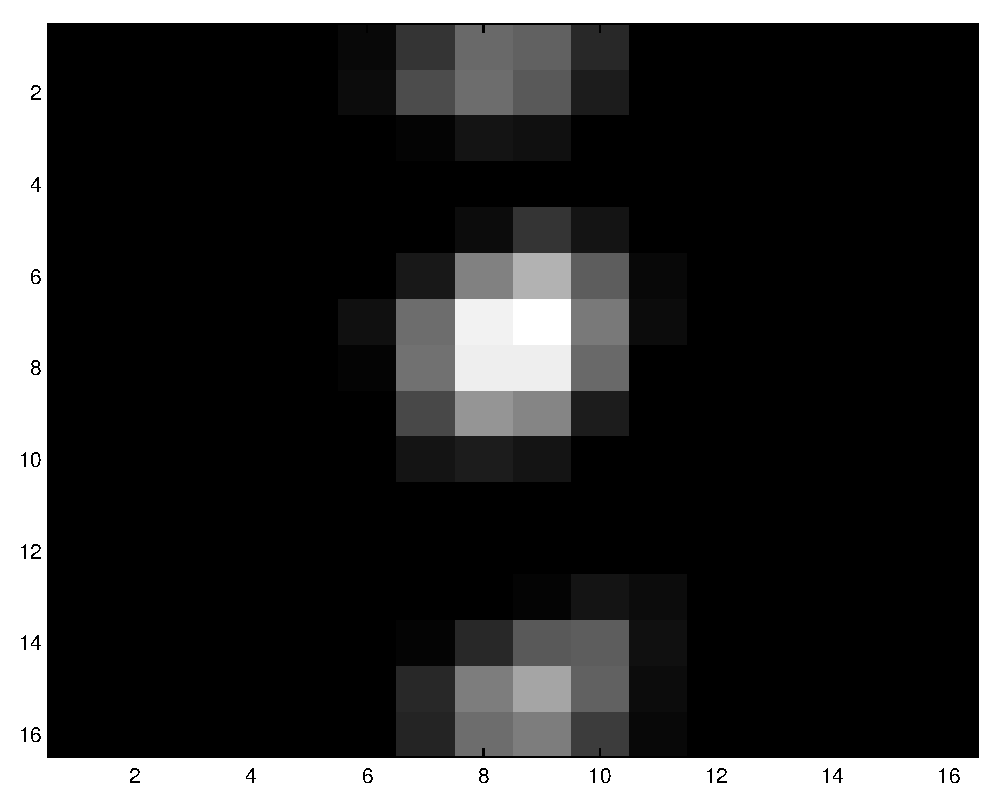
\includegraphics[width=0.25\textwidth]{codebook7.eps}\hspace{0.03\textwidth}%
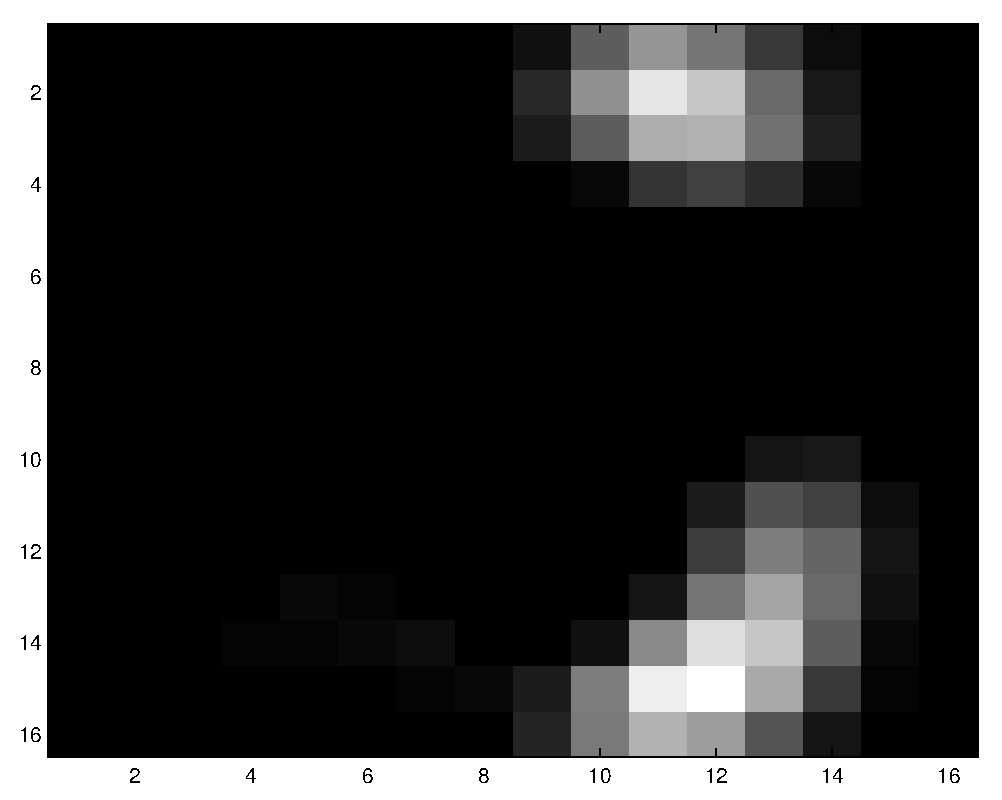
\includegraphics[width=0.25\textwidth]{codebook8.eps}\\[1em]
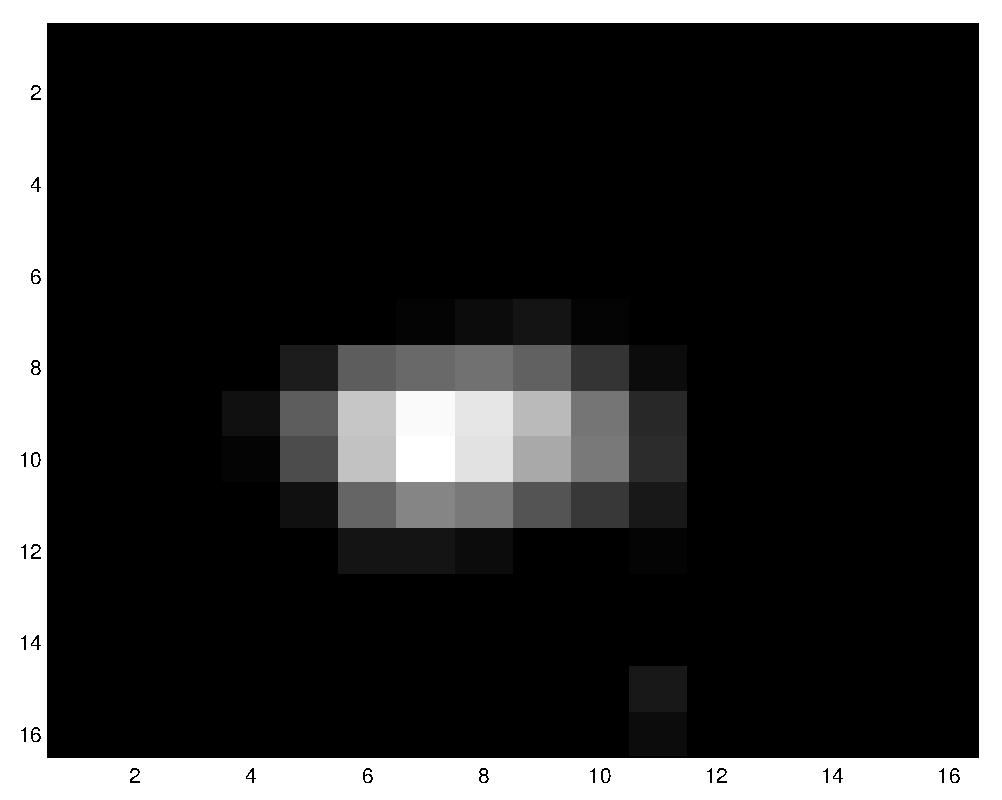
\includegraphics[width=0.25\textwidth]{codebook9.eps}\hspace{0.03\textwidth}%
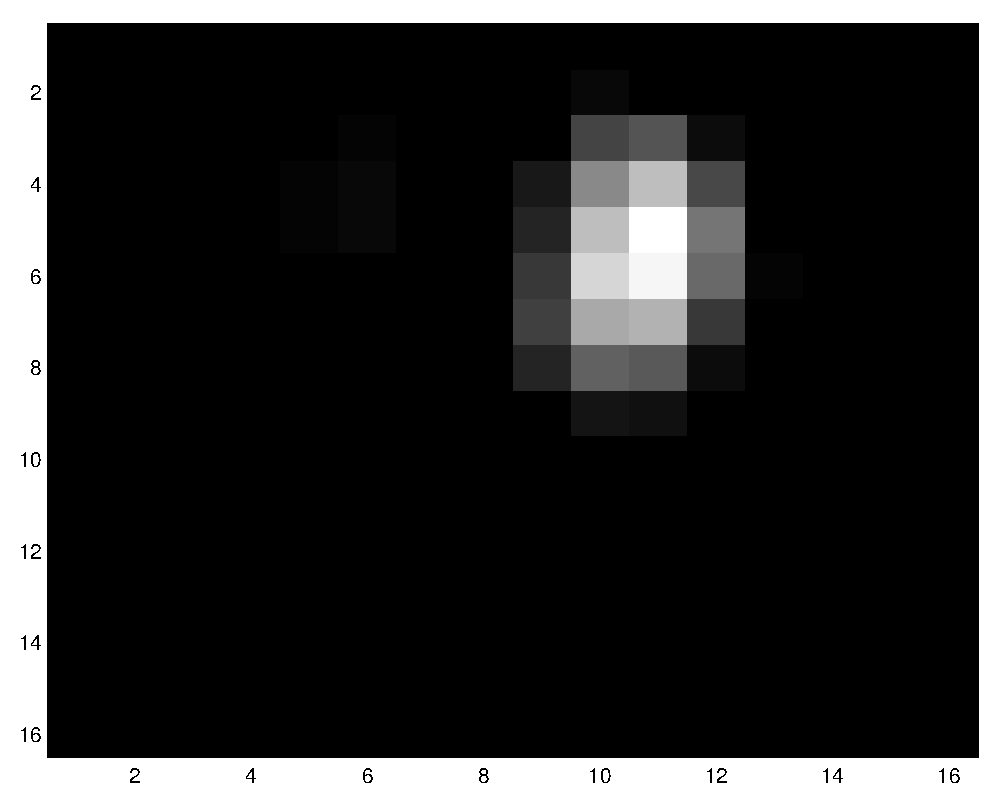
\includegraphics[width=0.25\textwidth]{codebook10.eps}\hspace{0.03\textwidth}%
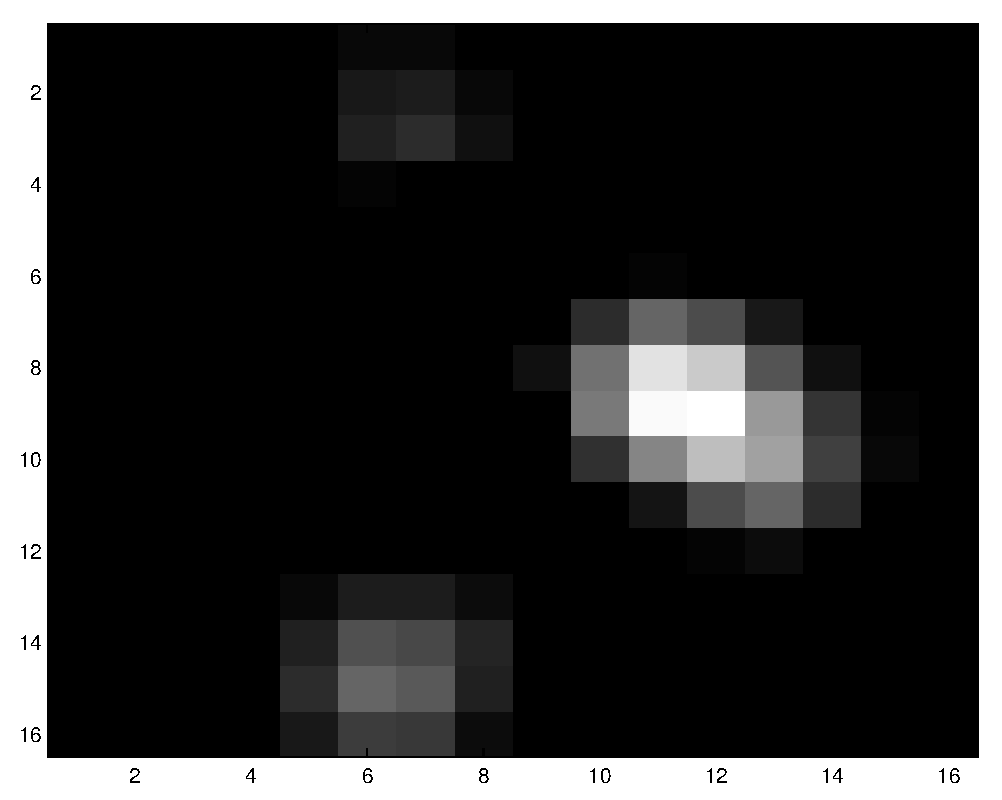
\includegraphics[width=0.25\textwidth]{codebook11.eps}\hspace{0.03\textwidth}%
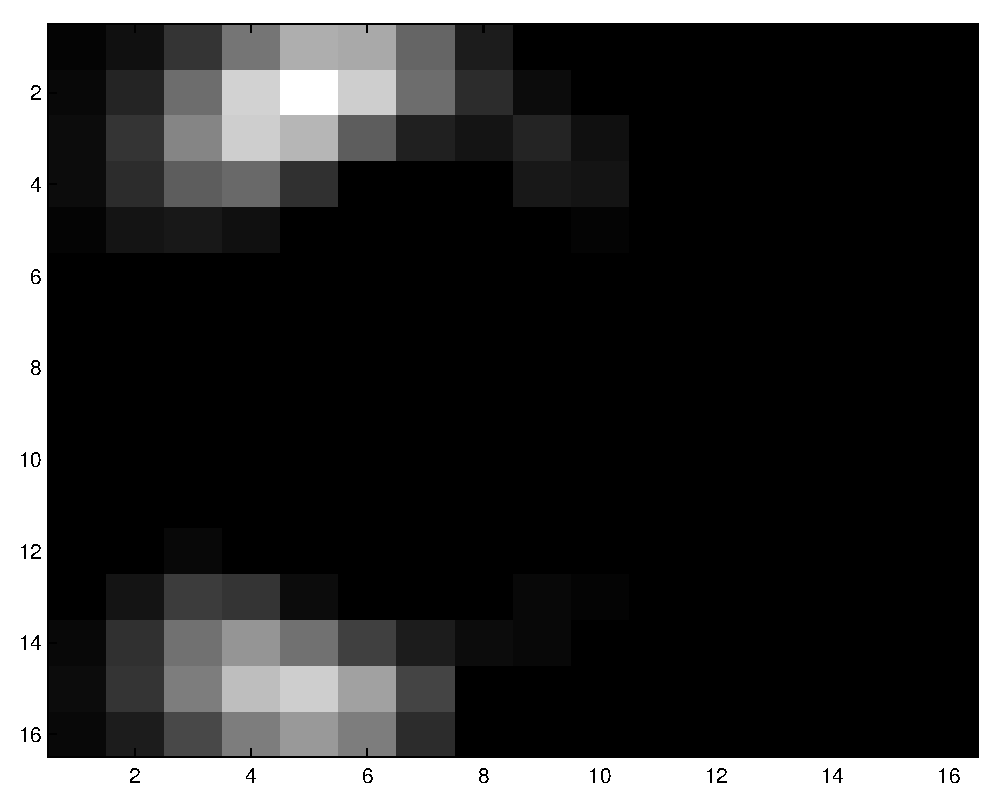
\includegraphics[width=0.25\textwidth]{codebook12.eps}\\[1em]
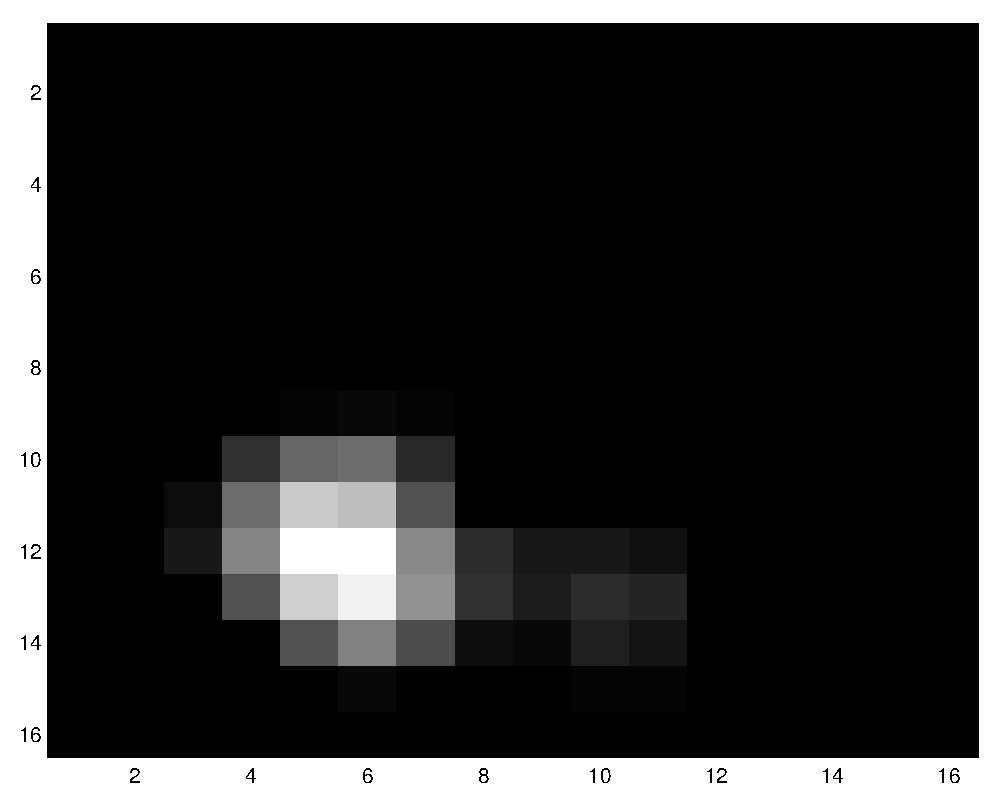
\includegraphics[width=0.25\textwidth]{codebook13.eps}\hspace{0.03\textwidth}%
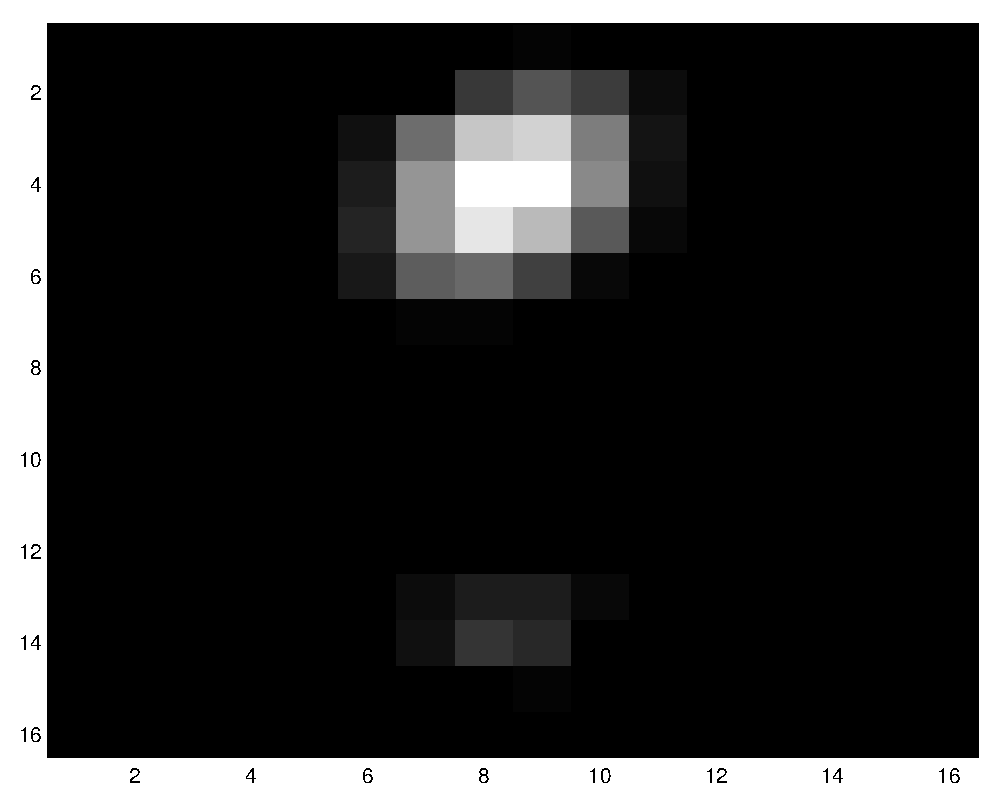
\includegraphics[width=0.25\textwidth]{codebook14.eps}\hspace{0.03\textwidth}%
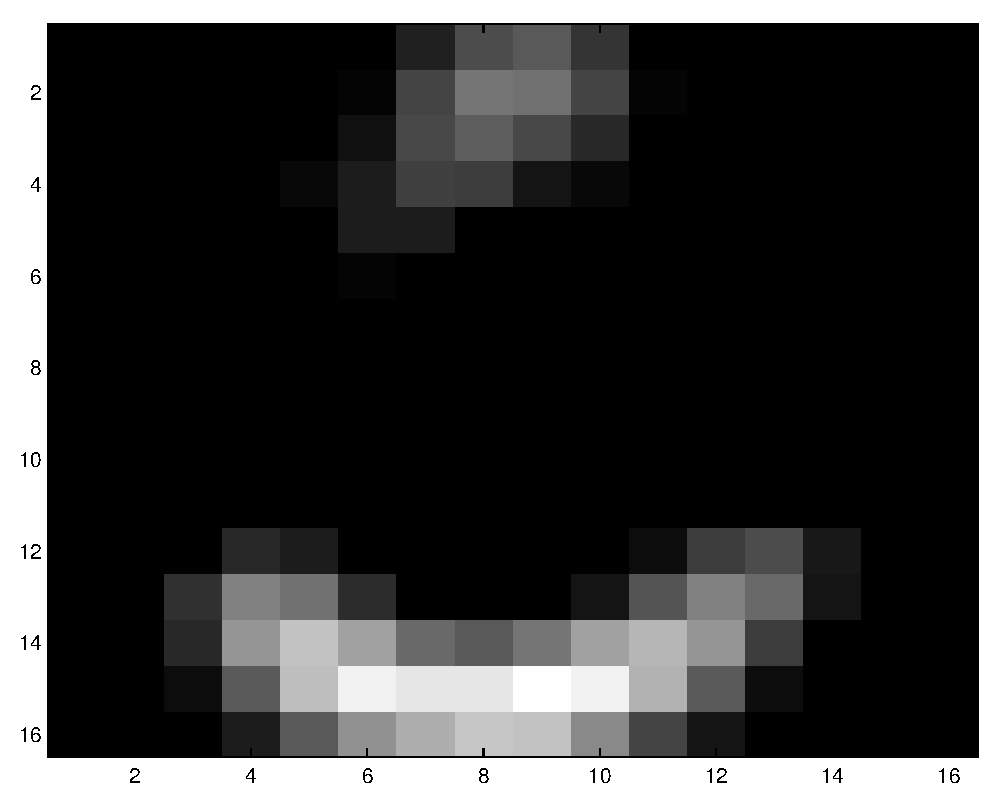
\includegraphics[width=0.25\textwidth]{codebook15.eps}\hspace{0.03\textwidth}%
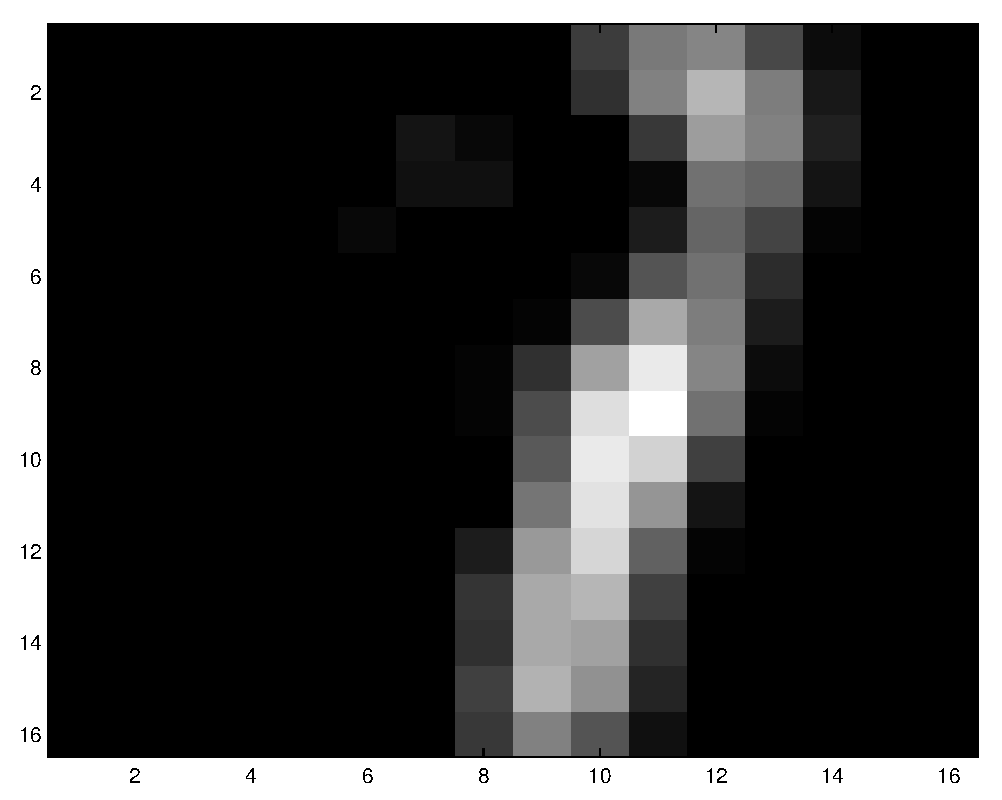
\includegraphics[width=0.25\textwidth]{codebook16.eps}\\[1em]
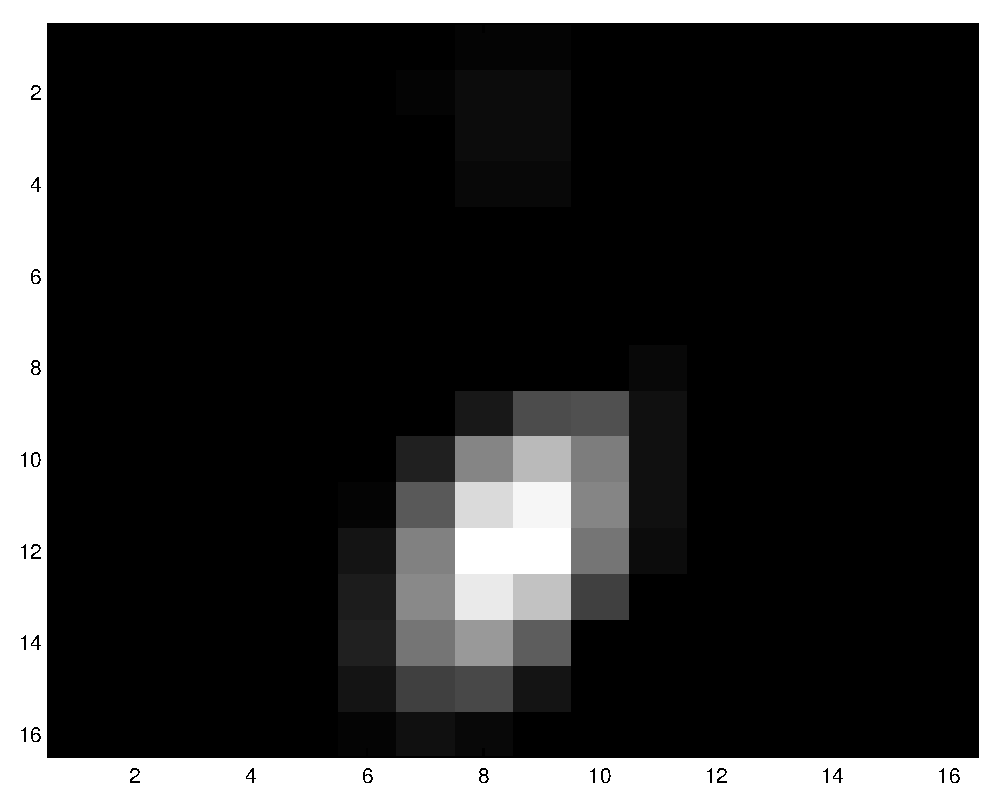
\includegraphics[width=0.25\textwidth]{codebook17.eps}\hspace{0.03\textwidth}%
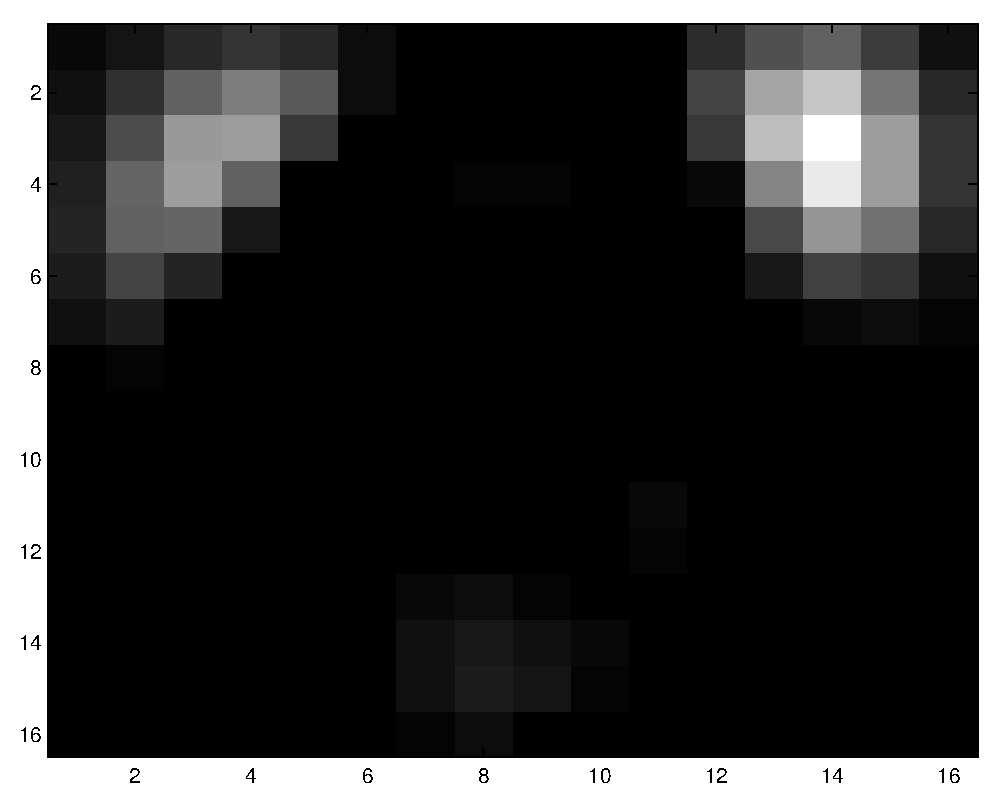
\includegraphics[width=0.25\textwidth]{codebook18.eps}\hspace{0.03\textwidth}%
\includegraphics[width=0.25\textwidth]{codebook19.eps}\hspace{0.03\textwidth}%
\includegraphics[width=0.25\textwidth]{codebook20.eps}\\[4em]
\newpage
Ein paar transformierte Testbilder:\\

\includegraphics[width=0.25\textwidth]{tes_original1.eps}\hspace{0.03\textwidth}%
\includegraphics[width=0.25\textwidth]{tes_original2.eps}\hspace{0.03\textwidth}%
\includegraphics[width=0.25\textwidth]{tes_original3.eps}\hspace{0.03\textwidth}%
\includegraphics[width=0.25\textwidth]{tes_original4.eps}\\[1em]
\includegraphics[width=0.25\textwidth]{H_tes1.eps}\hspace{0.03\textwidth}%
\includegraphics[width=0.25\textwidth]{H_tes2.eps}\hspace{0.03\textwidth}%
\includegraphics[width=0.25\textwidth]{H_tes3.eps}\hspace{0.03\textwidth}%
\includegraphics[width=0.25\textwidth]{H_tes4.eps}\\[1em]
\rule{1.09\textwidth}{0.4pt}\\[1em]
\includegraphics[width=0.25\textwidth]{tes_original5.eps}\hspace{0.03\textwidth}%
\includegraphics[width=0.25\textwidth]{tes_original6.eps}\hspace{0.03\textwidth}%
\includegraphics[width=0.25\textwidth]{tes_original7.eps}\hspace{0.03\textwidth}%
\includegraphics[width=0.25\textwidth]{tes_original8.eps}\\[1em]
\includegraphics[width=0.25\textwidth]{H_tes5.eps}\hspace{0.03\textwidth}%
\includegraphics[width=0.25\textwidth]{H_tes6.eps}\hspace{0.03\textwidth}%
\includegraphics[width=0.25\textwidth]{H_tes7.eps}\hspace{0.03\textwidth}%
\includegraphics[width=0.25\textwidth]{H_tes8.eps}\\[1em]


\end{document}
